\documentclass[10pt,landscape]{article}

\usepackage{multicol}
\usepackage{calc}
\usepackage{ifthen}
\usepackage[landscape]{geometry}
\usepackage{graphicx}
\usepackage{amsmath, amssymb, amsthm}
\usepackage{latexsym, marvosym}
\usepackage{pifont}
\usepackage{lscape}
\usepackage{graphicx}
\usepackage{array}
\usepackage{booktabs}
\usepackage{bm}  % bold math \bm{}
\usepackage[bottom]{footmisc}
\usepackage{tikz}
\usetikzlibrary{shapes}
\usepackage{pdfpages}
\usepackage{wrapfig}
\usepackage{enumitem}
\setlist[description]{leftmargin=0pt}
\usepackage{xfrac}
\usepackage[pdftex,
            pdfauthor={Janet Matsen},
            pdftitle={Machine Learning Cheatsheet},
            pdfsubject={Notes from UW CSE 446 Winter 2016},
            pdfkeywords={machine learning} {statistics} {cheatsheet} {pdf} {cheat} {sheet} {formulas} {equations}
            ]{hyperref}
\usepackage{relsize}
\usepackage{rotating}


 \newcommand\independent{\protect\mathpalette{\protect\independenT}{\perp}}
    \def\independenT#1#2{\mathrel{\setbox0\hbox{$#1#2$}%
    \copy0\kern-\wd0\mkern4mu\box0}} 
            
% Janet defined
\DeclareMathOperator*{\argmin}{arg\,min}
\DeclareMathOperator*{\argmax}{arg\,max}

% Probably from Stat cheatsheet:            
\newcommand{\noin}{\noindent}    
\newcommand{\logit}{\textrm{logit}} 
\newcommand{\var}{\textrm{Var}}
\newcommand{\cov}{\textrm{Cov}} 
\newcommand{\corr}{\textrm{Corr}} 
\newcommand{\N}{\mathcal{N}}
\newcommand{\Bern}{\textrm{Bern}}
\newcommand{\Bin}{\textrm{Bin}}
\newcommand{\Beta}{\textrm{Beta}}
\newcommand{\Gam}{\textrm{Gamma}}
\newcommand{\Expo}{\textrm{Expo}}
\newcommand{\Pois}{\textrm{Pois}}
\newcommand{\Unif}{\textrm{Unif}}
\newcommand{\Geom}{\textrm{Geom}}
\newcommand{\NBin}{\textrm{NBin}}
\newcommand{\Hypergeometric}{\textrm{HGeom}}
\newcommand{\HGeom}{\textrm{HGeom}}
\newcommand{\Mult}{\textrm{Mult}}

\geometry{top=.4in,left=.2in,right=.2in,bottom=.4in}

\pagestyle{empty}
\makeatletter
\renewcommand{\section}{\@startsection{section}{1}{0mm}%
                                {-1ex plus -.5ex minus -.2ex}%
                                {0.5ex plus .2ex}%x
                                {\normalfont\large\bfseries}}
\renewcommand{\subsection}{\@startsection{subsection}{2}{0mm}%
                                {-1explus -.5ex minus -.2ex}%
                                {0.5ex plus .2ex}%
                                {\normalfont\normalsize\bfseries}}
\renewcommand{\subsubsection}{\@startsection{subsubsection}{3}{0mm}%
                                {-1ex plus -.5ex minus -.2ex}%
                                {1ex plus .2ex}%
                                {\normalfont\small\bfseries}}
\makeatother

\setcounter{secnumdepth}{0}

\setlength{\parindent}{0pt}
\setlength{\parskip}{0pt plus 0.5ex}

% -----------------------------------------------------------------------

\usepackage{titlesec}

\titleformat{\section}
{\color{blue}\normalfont\large\bfseries}
{\color{blue}\thesection}{1em}{}
\titleformat{\subsection}
{\color{cyan}\normalfont\normalsize\bfseries}
{\color{cyan}\thesection}{1em}{}
% Comment out the above 5 lines for black and white

\begin{document}

\raggedright
\footnotesize
\begin{multicols*}{3}

% multicol parameters
% These lengths are set only within the two main columns
%\setlength{\columnseprule}{0.25pt}
\setlength{\premulticols}{1pt}
\setlength{\postmulticols}{1pt}
\setlength{\multicolsep}{1pt}
\setlength{\columnsep}{2pt}

%%%%%%%%%%%%%%%%%%%%%%%%%%%%%%%%%%%%
%%% TITLE
%%%%%%%%%%%%%%%%%%%%%%%%%%%%%%%%%%%%

\begin{center}
    {\color{blue} \Large{\textbf{Machine Learning Cheatsheet}}} \\
   % {\Large{\textbf{Probability Cheatsheet}}} \\
    % comment out line with \color{blue} and uncomment above line for b&w
\end{center}

%%%%%%%%%%%%%%%%%%%%%%%%%%%%%%%%%%%%
%%% ATTRIBUTIONS
%%%%%%%%%%%%%%%%%%%%%%%%%%%%%%%%%%%%

\scriptsize

Janet Matsen's Machine Learning (ML) notes from CSE 446, Winter 2016.  \url{http://courses.cs.washington.edu/courses/cse446/16wi/}

Used LaTeX template from an existing Statistics cheat sheet: \url{https://github.com/wzchen/probability_cheatsheet}, by William Chen (\url{http://wzchen.com}) and Joe Blitzstein. 

Licensed under \texttt{\href{http://creativecommons.org/licenses/by-nc-sa/4.0/}{CC BY-NC-SA 4.0}}. 

\begin{center}
    Last Updated \today
\end{center}

% Cheatsheet format from
% http://www.stdout.org/$\sim$winston/latex/

%%%%%%%%%%%%%%%%%%%%%%%%%%%%%%%%%%%%
%%% BEGIN CHEATSHEET
%%%%%%%%%%%%%%%%%%%%%%%%%%%%%%%%%%%%
  
    \hfill \\   
     \hfill \\  
\smallskip \hrule height 2pt \smallskip

\section{Essential ML ideas}
\smallskip \hrule height 2pt \smallskip

\begin{itemize}
	\item Never ever \underline{ever} touch the test set
	\item You know you are overfitting when there is a big test between train and test results.  E.g. metric of percent wrong. 
	\item Need to be comfortable taking a hit on fitting accuracy if you can get a benefit on the result.
	\item Bias vs variance trade-off.  
		High bias when the model is too simple \& doesn't fit the data well.  
		High variance is when small changes to the data set lead to large solution changes. 
	\item If features are non discriminative in the beginning, they don't work for any classifier.  % week 4 reminder
	\item Your feature vector often has a smaller dimension that the feature space.    % week 4, Friday. 
		If you have too long of a feature vector, you may get overfitting. 
	\item You need to prevent the optimizer from getting an easy way out.  % week 7 audio
\end{itemize}

You can do $l_2$ normalization for a feature vector to get a unit vector:   % week 6 audio. 
	Convert $x$ to $\hat{x}$ so that if you form $||\hat{x}||_2^2 = 1$
	Can also do $l_1$  


\section{Math/Stat Review}
\smallskip \hrule height 2pt \smallskip

\begin{description}
        \item[Random Variable X] belongs to set $\Omega$  
        \item[Conditional Probability \emph{is} Probability]  $P({A}|{ B})$ is a probability function for any fixed $B$. Any theorem that holds for probability also holds for conditional probability.   $P({A}|{ B}) = P(A \cap B)/P(B)$
        \item[Bayes' Rule] - Bayes' Rule unites marginal, joint, and conditional probabilities. We use this as the definition of conditional probability. 
        		\[P({\bf A}|{\bf B}) = \frac{P({\bf A} \cap {\bf B})}{P({\bf B})} = \frac{P({\bf B}|{\bf A})P({\bf A})}{P({\bf B})}\] 
		\[P(A = a \mid B) = \frac{P(A=a) P(B \mid A=a)}{\sum\limits_{a'} P(A=a) P(B \mid A=a)} \]   % TA lecture 1/7/2015
        \item[Law of Total Probability]: $\sum\limits_x P(X=x) = 1$
        \item[Product Rule]: $P(A,B) = P(A \mid B) \cdot P(B)$  % TA lecture 1/7/2015
        \item[Sum Rule]: $P(A) = \sum\limits_{x \in \Omega} P(A, B=b)$  % TA lecture 1/7/2015
        \item[i.i.d]: $D=\{x_i | i=1 \dots n\}, P(D | \theta) = \prod_i P(x_i \mid \theta)$
\end{description}

Vocab:
\begin{itemize}
	\item \textbf{likelihood function} $L(\theta | O)$ is called as the likelihood function. $\theta$ = unknown parameters, $O$ is the observed outcomes.  The likelihood function is conditioned on the observed $O$ and that it is a function of the unknown parameters $\theta$.  Not a probability density function.
	\item \textbf{"likelihood" vs "probability"}: if discrete, $L(\theta | O)= P(O | \theta)$.  If continuous, $P(O|\theta)=0$ so instead we estimate $\theta$ given $O$ by maximizing $L(\theta | O)= f(O | \theta)$ where $f$ is the pdf associated with the outcomes $O$. 
		% http://stats.stackexchange.com/questions/2641/what-is-the-difference-between-likelihood-and-probability
	\item \textbf{hypothesis space}
\end{itemize} 

\subsection{Law of Total Probability (LOTP)}  % from cheat sheet: https://github.com/wzchen/probability_cheatsheet/blob/master/probability_cheatsheet.tex
Let ${ B}_1, { B}_2, { B}_3, ... { B}_n$ be a \emph{partition} of the sample space (i.e., they are disjoint and their union is the entire sample space).
\begin{align*} 
    P({ A}) &= P({ A} | { B}_1)P({ B}_1) + P({ A} | { B}_2)P({ B}_2) + \dots + P({ A} | { B}_n)P({ B}_n)\\
    P({ A}) &= P({ A} \cap { B}_1)+ P({ A} \cap { B}_2)+ \dots + P({ A} \cap { B}_n)
    \end{align*} 
    For \textbf{LOTP with extra conditioning}, just add in another event $C$!
    \begin{align*} 
    P({ A}| { C}) &= P({ A} | { B}_1, { C})P({ B}_1 | { C}) + \dots +  P({ A} | { B}_n, { C})P({ B}_n | { C})\\
    P({ A}| { C}) &= P({ A} \cap { B}_1 | { C})+ P({ A} \cap { B}_2 | { C})+ \dots +  P({ A} \cap { B}_n | { C})
\end{align*} 

Special case of LOTP with ${ B}$ and ${ B^c}$ as partition:
   \begin{align*} 
P({ A}) &= P({ A} | { B})P({ B}) + P({ A} | { B^c})P({ B^c}) \\
P({ A}) &= P({ A} \cap { B})+ P({ A} \cap { B^c}) \\
   \end{align*} 
   
\subsection{Bayes' Rule}  % from cheat sheet: https://github.com/wzchen/probability_cheatsheet/blob/master/probability_cheatsheet.tex

\textbf{Bayes' Rule, and with extra conditioning (just add in $C$!)}
         \[P({ A}|{ B})  = \frac{P({ B}|{ A})P({ A})}{P({ B})}\]
         \[P({ A}|{ B}, { C}) = \frac{P({ B}|{ A}, { C})P({ A} | { C})}{P({ B} | { C})}\]
         We can also write
         $$P(A|B,C) = \frac{P(A,B,C)}{P(B,C)} = \frac{P(B,C|A)P(A)}{P(B,C)}$$
\textbf{Odds Form of Bayes' Rule}
\[\frac{P({ A}| { B})}{P({ A^c}| { B})} = \frac{P({ B}|{ A})}{P({ B}| { A^c})}\frac{P({ A})}{P({ A^c})}\]
The \emph{posterior odds} of $A$ are the \emph{likelihood ratio} times the \emph{prior odds}. 
\hfill \\ \hfill \\

Practice:  What is $P(disease \mid + test)$ if P(disease) = 0.01, \hfill \\  % TA lecture 1/7/2015
  P(+ $\mid$ disease) = 0.99, P(+ $\mid$ no disease) = 0.01? 
% ANS: P(disease | +) = P(-d)*P(+ | d) / (P(-d)*P(+|-d) + P(d)*P(+ | -d)

\subsection{Expectation}  % TA lecture 1/7/2015
\begin{description}
        \item[f(X)] probability distribution function of X  % TA lecture 1/7/2015
        \item[X $\sim$ P]: X is distributed according to P.   % TA lecture 1/7/2015
        \item[Expected value of f under P]: $E_{P}[f(x)] = \sum\limits_{x} p(x)f(x)$
\end{description} 

E.g. unbiased coin.  x = {1, 2, 3, 4, 5, 6}.  p(X=x) = 1/6 for all x.  \hfill \\
E(X) = $\sum\limits_{x} p(x) \cdot x = (1/6) \cdot [1 + 2 + 3 + 4 + 5 + 6] = 3.5$

\subsection{Entropy}
Always greater than  or equal to 0.  Zero when outcome is certain.  1 for uniform distribution. \hfill \\
Entropy is based on a pdf, not a list of labels. E.g.  \hfill \\
H[1,1,0] $\rightarrow$ H[2/2, 1/3]. 

$X \sim P$, $x \in \Omega$  \hfill \\

\hfill \\
First define \textbf{Surprise}: $S(x) = -\log_2 p(x)$   \hfill \\
$S(X = \mbox{heads}) = -\log_2 (1/2) = 1 $.     \hfill \\
\begin{description}  % http://www.cs.cmu.edu/~venkatg/teaching/ITCS-spr2013/notes/15359-2009-lecture25.pdf
        \item[Axiom 1]: S(1) = 0. (If an event with probability 1 occurs, it is not surprising at all.)  
        \item[Axiom 2]: S(q) $>$ S(p) if q $<$ p. (When more unlikely outcomes occur, it is more surprising.)  
        \item[Axiom 3]: S(p) is a continuous function of p. (If an outcome�s probability changes by a tiny
amount, the corresponding surprise should not change by a big amount.)
	\item[Axiom 4]: S(pq) = S(p) $+$ S(q). (Surprise is additive for independent outcomes.)
\end{description}
Surprise of 7 = pretty surprised.  Probability of $1/2^7$ of happening
\hfill \\ 

(Shannon) \textbf{Entropy}:   
% http://www.cs.cmu.edu/~venkatg/teaching/ITCS-spr2013/notes/15359-2009-lecture25.pdf
\begin{align*}
	H[X] &= - \sum\limits_x p(x) \cdot \log_2 p(x) \\
		&= - \sum\limits_x p(x) S(x)  \\
		&= E[S(x)]  
\end{align*}
The entropy is the expectation of the surprise.  Throw out x for $p(x)=0$ because log(0) is $\infty$. \hfill \\
\hfill \\
\underline{Binary Entropy Function}:  $p(X = 1) = \theta$ and $p(X = 0) = 1 - \theta$
\begin{align*}
	H(X) &= - [p(X=1) \log_2 p(X=1)+p(X=0) \log_2 p(X=0)]  \\
		& = - [\theta \log_2 \theta+(1 - \theta) \log_2(1 - \theta)]
\end{align*}
\hfill \\

\underline{Entropy of an unbiased coin flip:} \hfill \\
X is a coin flip. $P(X=\mbox{heads}) = 1/2$, $P(X=\mbox{tails}) = 1/2$  \hfill \\
Note: $\log_2(1/2) = -1$, $- \log_2(1/2) = \log_2(2) = 1$   \hfill \\
$H[X] = -[1/2 \log_2(1/2) + 1/2 \log_2(1/2)] = 1$   \hfill \\
\hfill \\
\underline{Entropy of a coin that always flips to heads:} \hfill \\
$P(X=\mbox{heads}) = 1$, $P(X=\mbox{tails}) = 0$  \hfill \\
Note: $\log_x(0) = 0$   \hfill \\
$H[X] = -[1 \log_2(1) + 0] = 0$   \hfill \\
No surprise: you are sure what you are going to get.  \hfill \\
 \hfill \\

Binary entropy plot. 
\begin{minipage}{\linewidth}
\begin{center}
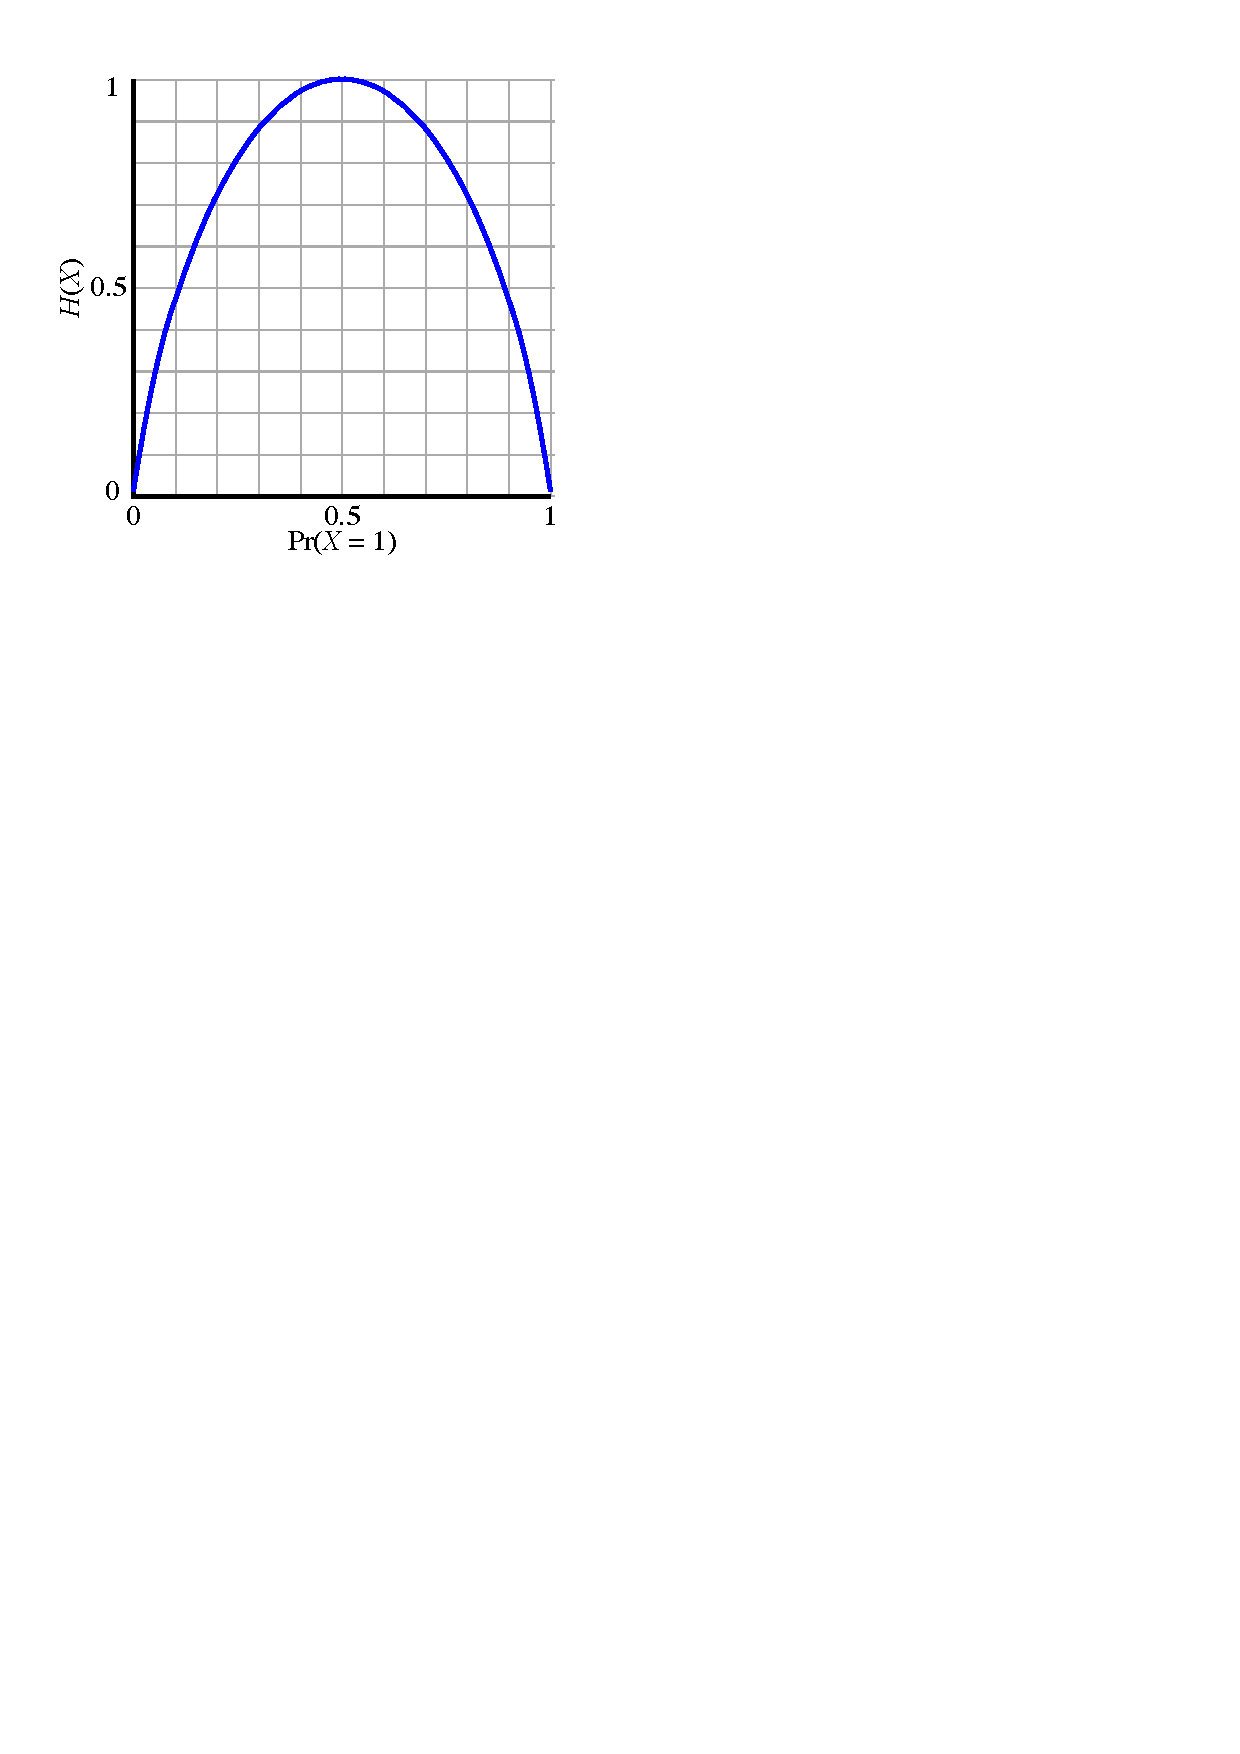
\includegraphics[width=1.3in]{figures/Binary_entropy_plot.pdf}
\end{center}
\end{minipage}

\underline{Canonical example:} \hfill \\  % TA lecture 1/7/2015. 
\begin{tabular}{ l | r }
  X & Y \\ \hline
  0 & 1 \\
  1 & 0 \\
  1 & 1 \\
\end{tabular}
\hfill \\
If you want to estimate entropy of X, you can use P(X=0).  \hfill \\
\begin{align*}
	H[X] &= -[\frac{1}{3} \log_2 \frac{1}{3} + \frac{2}{3} \log_2 \frac{2}{3}] \\
		& = \frac{1}{3} \log_2 3 + \frac{2}{3} \log_2 3 - \frac{2}{3} \log_2 2 \\
		&= \log_2 3 - \frac{2}{3} \approx 0.91
\end{align*}
This time H[X] = H[Y] because of symmetry.  \hfill \\

The discrete distribution with maximum entropy is the uniform distribution.  For K values of X, $H(X) = \log_2 K$ \hfill \\  % book pg 57
Conversely, the distribution with minimum entropy (which is zero) is any delta-function that puts all its mass on one state. Such a distribution has no uncertainty. 
\hfill \\

\subsection{Conditional Entropy}
If you don't know x:  (this is kind of an average).  \hfill \\
$H[Y \mid X=x] = -\sum\limits_y P(Y=y \mid X=x) \cdot \log_2 P(y \mid X=x)$   \hfill \\
 $H[Y \mid X=x] =  E[S(Y \mid X=x)]  $  \hfill \\
Note that we are summing over y because we are specifying x. \hfill \\
\hfill \\

For a particular value of X:  \hfill \\
$H[Y \mid X] = \sum\limits_x p(x) H[Y \mid X=x]$  \hfill \\
\hfill \\

Back to table above: 
\begin{align*}
	H[Y \mid X=0] &= ?  \\
	& \mbox{look only at X=0 in table.}  \\
	&= -[0 + 1 \log_2]  \\
\end{align*}
Now that you know X=0, entropy goes to 0.   \hfill \\  \hfill \\

$H[Y \mid X=1] = 1$: You know \textit{less} if you know X=1. \hfill \\ \hfill \\

Now use 
$H[Y \mid X] = \frac{1}{3}(0) + \frac{2}{3}(1) = 2/3$ \hfill \\
Given X, you know more.  Average our the more certain case and the less certain case.  \hfill \\  \hfill \\

Note:  $H[Y \mid X] \leq H[Y]$: knowing something can't make you know less. 

\subsection{Entropy and Information Gain}
\textbf{Information Gain} -  $IG(X) = H(Y) - H(Y \mid X)$ \hfill \\
Y is the node on top.  X are the nodes below.  He might have used lower case.  \hfill \\
\textbf{Class Example}: If $X_1$ is a node for a split, and you want to know the information gain for that node, you:
\begin{itemize}
	\item calculate entropy of the split.  Find Entropy of each branch of the split, and the fraction of points that were channeled to each split.  E.g. %http://courses.cs.washington.edu/courses/cse446/16wi/Slides/2_DecisionTrees_Part2.pdf
	\begin{align*}
		\{T, T, T, T, T, F\} & \rightarrow \{T, T, T, T\} \mbox{ (for } X_1=T), \{T, F\} \mbox{ (for } X_1=F) \\
				& \rightarrow P(X_1 = T) = 4/6, P(X_1=F) = 2/6 \\
				& \rightarrow H(X_1 = T) =  (1*\log_2 1 + 0*\log_2 0) = 0 \\
				& \rightarrow H(X_1 = F) =  \frac{2}{6} (\frac{1}{2} \log_2 \frac{1}{2} + \frac{1}{2} \log_2 \frac{1}{2})  \\
				& = 1 \mbox{ (uniform distribution)} \\
				H(Y|X_1)  =  - \frac{4}{6} & (1*\log_2 1 + 0*\log_2 0) - \frac{2}{6} (\frac{1}{2} \log_2 \frac{1}{2} + \frac{1}{2} \log_2 \frac{1}{2}) \\
							& = 2/6
	\end{align*}
	\item find the entropy of the unsplit data:  $\{T, T, T, T, T, F\} \rightarrow -(5/6) \log_2(5/6) - (1/6) \log_2(1/6) = 0.65$  % check w/ google: -(5/6)*log_2(5/6) - (1/6)*log_2(1/6) == 0.65. 
	\item subtract the weighted average of the split entropies from the original: $IG(X_1) = H(Y) - H(Y|X_1) = 0.65 - 0.33$
\end{itemize}


%\textbf{Conditional Information Gain}:    \hfill \\ %$H(y|x) = -\sum P(y|x) log_2$ 
  \hfill \\

\begin{itemize}
	\item Low uncertainty $\leftrightarrow$ Low entropy.
	\item Lowering entropy $\leftrightarrow$ More information gain. 
\end{itemize}


\subsection{Bits}
If you use log base 2 for entropy, the resulting units are called bits (short for binary digits). \hfill \\ % book pg 57
How many things can you encode in 15 bits? $2^{25}$.  \hfill \\  % 1/11/2015 Lecture


\subsection{Common notation}
\textbf{semicolon versus $|$ in probabilities}: \hfill \\
E.g. $P(X ; \theta)$ vs $P(X | \theta)$

$|$ is for random variables and $;$ is for parameters.  

Andrew Ng verbalizes the semicolon as "parameterized by."  
So $f(x ; \theta)$ would be spoken as "f of x parameterized by theta"
	






\section{Decison Trees}
\smallskip \hrule height 2pt \smallskip



\section{Maximum Likelihood \& Maximum a Posteriori}
\smallskip \hrule height 2pt \smallskip

\underline{Vocab}
\begin{itemize}
	\item\textbf{likelihood}: the probability of the data given a parameter.  E.g. $P(D | \theta)$ (for discrete like Binomial).  
	Need not a pdf; need not be normalized.   %  http://www.robots.ox.ac.uk/~az/lectures/est/lect34.pdf  + Erick
 	\item \textbf{log-likelihood}: lower-case: $l(\theta|x) = \log L(\theta | x)$
	\item \textbf{MLE}: Maximum Likelihood Estimation. 
	\item \textbf{PAC}: Probability Approximately Correct. 
\end{itemize}

\underline{ML}: Maximum Likelihood \hfill \\
 \hfill \\
 
\underline{MLE}: Maximum Likelihood Estimation \hfill \\
Choose $\theta$ to maximize probability of D. \hfill \\
Set derivative of \_\_ to zero and solve.  If function is multivariate, set each partial derivative to zero and solve. \hfill \\
$\hat{\theta} = \argmax_\theta P(D | \theta) = \argmax_\theta \ln P(D | \theta) $ \hfill \\
Note we are using $\ln$, not $\log_2$ as we did for entropy above.  Want it to cancel exponents now. 
 \hfill \\
 
\hfill \\
\underline{Binomial Distribution} \hfill \\
Assumes i.i.d: $D=\{x_i | i=1 \dots n\}, P(D | \theta) = \prod_i P(x_i \mid \theta)$. \hfill \\
Likelihood function: $P(D | \theta) = \theta^{\alpha_H} (1-\theta)^{\alpha_T}$  \hfill \\
P(heads) = $\theta$, P(tails) = $1 - \theta$ \hfill \\
\begin{align*} 
	\hat{\theta} &= \argmax_\theta \ln P(D| \theta) \\
	 	 &= \argmax_\theta \ln \theta*{\alpha H}(1-\theta)^{\alpha T}
\end{align*}
Find optimal theta by setting the derivative to zero: 
\begin{align*} 
	\frac{d}{d\theta} \ln P(D| \theta) &= \frac{d}{d\theta}  \ln \theta*{\alpha H}(1-\theta)^{\alpha T} \\
	 	 &= \argmax_\theta \ln \theta*{\alpha H}(1-\theta)^{\alpha T} \\
		 & = \dots = \frac{\alpha_H}{\alpha_H  + \alpha_T}
\end{align*}

For Binomial, there is exponential decay in uncertainty with \# of observations.  % slide 7 at http://courses.cs.washington.edu/courses/cse446/16wi/Slides/3_PointEstimation.pdf
You can also find the probability that you are approximately correct (see \href{http://courses.cs.washington.edu/courses/cse446/16wi/Slides/3_PointEstimation.pdf}{notes}).  \hfill \\
$P(|\widehat{\theta} = \theta*| \geq \epsilon) \leq 2e^{-2N\epsilon^2}$.  Can calculate N (\# of flips) to have error less than $\epsilon$ with probability of being incorrect $\delta$.  Your sensitivity depends on your problem; error on stock market data might cost billions. 

What if you had prior beliefs?  Use MAP instead of MLE.



\section{Bayesian Learning}
\smallskip \hrule height 2pt \smallskip

Rather than estimating a single $\theta$, we obtain a  distribution over possible values of $\theta$.

For small sample size, prior is important! 

Use Bayes' Rule:
$ \displaystyle P(\theta | D) = \frac{P(D | \theta) P(\theta)}{P(D)}$
\begin{itemize}
	\item \textbf{Posterior}: $P(\theta | D)$
	\item \textbf{Data Likelihood}: $P(D | \theta) $
	\item \textbf{Prior}: $P(\theta)$
	\item \textbf{normalization}: $P(D)$
\end{itemize}
Or equivalently, $P(\theta | D) \propto P(D | \theta) P(\theta)$

If you have a uniform prior, you just do MLE.  \hfill \\
$P(\theta) \propto 1 \rightarrow P(\theta | D) \propto P(D | \theta)$

\underline{Vocab}
\begin{itemize}
	\item \textbf{prior}: 
	\item \textbf{prior distribution}: 
	\item \textbf{posterior}: 
	\item \textbf{posterior distribution}: 
	\item \textbf{MAP}:
\end{itemize}

\hfill \\
\underline{Thumbtack Problem}
\begin{itemize}
	\item use Binomial likelihood:  $P(D | \theta) = \theta^{\alpha_H} (1-\theta)^{\alpha_T}$
	\item To get a simple posterior form, use a conjugate prior.  Conjugate prior of Binomial is the Beta Distribution.  See \href{http://courses.cs.washington.edu/courses/cse446/16wi/Slides/3_PointEstimation.pdf}{slides} for math. 
	\item The Beta prior is equivalent to extra thumbtack flips.  As $N \rightarrow \infty$, the prior is �forgotten�.  But for small sample size, prior is important.  
\end{itemize}

If you are measuring a continuous variable, Gaussians are your friend. 

\section{Gaussians}
\smallskip \hrule height 2pt \smallskip

Properties of Gaussians: 
\begin{itemize} 
	\item Affine transformation (multiplying by a scalar and adding a constant) are Gaussian.
		If X $\sim$ N($\mu$,$\sigma^2$) and Y = aX + b, then Y $\sim$ N($a\mu+b, a^2\sigma^2$) 
  	\item Sum of Gaussians is Gaussian.  
			If X $\sim$ N($\mu_X, \sigma^2_X$), 
			Y $\sim$ N($\mu_Y, \sigma^2_Y$), 
			and Z = X+Y, then 
			Z $\sim$ N($\mu_X+\mu_Y, \sigma_X^2 +\sigma_Y^2$)
	\item  Easy to differentiate.
\end{itemize}

Learn a Gaussian: $P(x | \mu, \sigma) = \frac{1}{\sigma \sqrt{2 \pi}}e^\frac{-(x-\mu)^2}{2\sigma^2}$. \hfill \\
MLE for Gaussian: Prob of i.i.d. samples D = $\{x_1, \dots, x_N\}$:  \hfill \\
$\displaystyle  P(D|\mu, \sigma) = ( \frac{1}{\sigma \sqrt{2 \pi}})^N \prod_{i=1}^N e^\frac{-(x_i-\mu)^2}{2\sigma^2}$.   \hfill \\
Note: it is \underline{not} $P(\mu, \sigma | D)$, like I thought in class.  \hfill \\
Find $\mu_{MLE}$, $\sigma_{MLE} = \argmax_{\mu, \sigma} P(D | \mu, \sigma)$.  \hfill \\

Log-likelihood:  $ \displaystyle \ln P(D | \mu, \sigma) = \ln[\mbox{thing above}] = -N \ln \sigma \sqrt{2\pi} - \sum_{i=1}^N \frac{(x_i - \mu)^2}{2\sigma^2}$.  \hfill \\
Differentiate w.r.t. $\mu$ and set = 0.  End up with $ \displaystyle \widehat{\mu} = \frac{1}{N} \sum_{i=1}^N x_i$.  \hfill \\
Differentiate w.r.t. $\sigma$ and set = 0.  End up with $ \displaystyle \widehat{\sigma}^2_{MLE} = \frac{1}{N} \sum_{i=1}^N (x_i-\widehat{\mu})^2$.  \hfill \\
But actually, that leads to a biased estimate, so people actually use  $ \displaystyle \widehat{\sigma}^2_{unbiased} = \frac{1}{N-1} \sum_{i=1}^N (x_i-\widehat{\mu})^2$  \hfill \\

The conjugate priors: mean: use Gaussian prior:  $ \displaystyle  P(\mu | \nu, \lambda) = \frac{1}{\lambda \sqrt{2 \pi}}e^\frac{-(\mu - \nu)^2}{2\sigma^2} $.  (Instead of $\sigma$, use $\lambda$ and replace the $(x-\mu)^2$ with $(\mu - \nu)^2$).  \hfill \\
For variance: use Wishard Distribution:  

\section{Linear Regression}
\smallskip \hrule height 2pt \smallskip

The loss is $|| y - Xw ||^2 + \lambda || w ||^2$ \hfill \\
(this corresponds to the sum of squared error loss + L2 regularization)\hfill \\
\hfill \\

\underline{Ordinary Least Squares} \hfill \\

Notation:
\begin{itemize}
	\item \textbf{$x_i$}: an input data point.  \_\_ rows by \_\_ columns. 
	\item \textbf{$y_i$}: a predicted output
	\item \textbf{$\widehat{y_i}$}: a predicted output
	\item \textbf{$\widehat{y}$}: 
	\item \textbf{$w_k$}: weight k
	\item \textbf{$\bm{w}^*$}: the vector of weights found in regression.   
	\item \textbf{$f_k(x_i)$}
	\item \textbf{$t$}: what we want to regress against
	\item \textbf{$t_j$}: the output variable that you either have data for or are predicting. 
	\item \textbf{$t(\bm{x})$}: Data.  "Mapping from x to t(x)"
	\item \textbf{$H$}: $H = \{ h_1, \dots, h_K \}$.  Basis functions.  In the simplest case, they can just be the value of an input variable/feature or a constant (for bias).  
	\item \textbf{$L_2$}: The $L_2$.  Can appear as a loss function to describe the deviation from data or as a penalty.  
		% Erick clarification
	\item \textbf{$ || \widehat{w} ||_1$}: "$L_1$" penalty.  The "Manhattan distance".  Like traveling a, b in a pythagorean triangle.  $\sum |x_i|$
	\item \textbf{$ || \widehat{w} ||_2$}.  "$L_2$" penalty.  Euclidean length of a vector.  Like c in a pythagorean triangle.  $\sqrt{\sum |x_i|^2}$	
\end{itemize}

\underline{Vocab}:
\begin{itemize}
	\item \textbf {bias-variance tradeoff} - the problem of simultaneously minimizing two sources of error that prevent 
			supervised learning algorithms from generalizing beyond their training set.  % https://en.wikipedia.org/wiki/Bias%E2%80%93variance_tradeoff
			\begin{itemize}  
				\item The bias is error from erroneous assumptions in the learning algorithm. 
					High bias can cause an algorithm to miss the relevant relations between features 
					and target outputs (underfitting).
				\item The variance is error from sensitivity to small fluctuations in the training set. 
					High variance can cause overfitting: modeling the random noise in the training 
					data, rather than the intended outputs.
			\end{itemize}
	\item \textbf{basis function}
	\item \textbf{bias} (parameter): like the intercept in a linear equation.  The part that doesn't depend on the features. 
	\item \textbf{bias} (learning bias):  (?? "inductive bias" ??)  - 
	\item \textbf{hyperplane} - a plane, usually with more than 2 dimensions. 
	\item \textbf{input variable} - a.k.a. feature.  % https://en.wikipedia.org/wiki/Dependent_and_independent_variables
		E.g. a column like CEO salary for rows of data corresponding to different companies.
	\item \textbf{response variable} - synonyms: "dependent variable", "regressand", "predicted variable", "measured variable", "explained variable", "experimental variable", "responding variable", "outcome variable", and "output variable".   E.g. a predicted stock price.   
	\item \textbf{regularization} -  introducing additional information in order to solve an ill-posed problem or to prevent overfitting. 
	% https://en.wikipedia.org/wiki/Regularization_(mathematics)
	E.g. applying a penalty for large parameters in the model. 
	\item \textbf{ridge regression} - 
	\item \textbf{vector norm}: put in a vector and get out a number like length or size.  Real valued function of some sort of vector or matrix quantity. 
	\item \textbf{hyperparameters}: \hfill \\
	$\lambda$, not $w$.  Parameters that control your actual parameters.  \hfill \\ \hfill \\
	% Wrong?!?   Norm 1 and norm 2 are not "parameters".  $\dots$ model design.  \hfill \\
	% Wrong?!?   Different values of lambda won't change the complexity of the model.  \hfill \\

	% Erick definition:
	In Bayesian analysis, the parameters that don't touch the data.  
	Like the parameters for the prior on the prior.  
	Called the ridge regression $\lambda$ a hyperparameter, though this is a stretch in the terminology.  \hfill \\
	Class version: 
	\item \textbf{feature selection}: explicitly select features that can go into your model instead of throwing all features in. 
	\item \textbf{loss function}:  
		% wikipedia:
		 A function that maps an event or values of one or more variables onto a real number intuitively representing some 			"cost" associated with the event. 
		 An optimization problem seeks to minimize a loss function. \hfill \\
		% week 4 typed notes near bottom. 
		$\sum_j (t(x_j) - \sum w_i h(x_i))^2$. (least-squares error ($L_2$))  (??? = training error??)
	\item \textbf{training set error}:  *doesn't include the regularization penalty!*.  A.k.a. "training error".  
			Sum of squares error divided by the number of points.   See formula later. 
%	\item \textbf{training error}:  sononomous
\end{itemize}

\subsection{Ordinary Least Squares}
total error = $\displaystyle \sum_i (y_i-\hat{y_i})^2 = \sum_i(y_i - \sum_k w_k f_k(x_i))^2$ \hfill \\
$i$ is for each data point, $k$ is for each of the k basis functions. 

 \hfill \\ \hfill \\

Under the additional assumption that the errors be normally distributed, OLS is the maximum likelihood estimator. \hfill \\ % https://en.wikipedia.org/wiki/Ordinary_least_squares
?? Use words to describe what subset of regression in general this is.  What is ordinary? What are we limiting?  \hfill \\
 \hfill \\

The regression problem: \hfill \\
Given basis functions $\{ h_1, \dots, h_K \}$  with $h_i(\bf{x}) \in \mathbb{R}$,  \hfill \\
	find coefficients $\bm{w} = \{ w_1, \dots, w_k \}$.  \hfill \\%  
$t(\bm{x}) \approx \widehat{f}(\bm{x}) = \sum_i w_i h_i(\bm{x})$     \hfill \\  \hfill \\


This is called linear regression b/c it is linear in the parameters. 
We can still fit to nonlinear functions by using nonlinear basis functions;  $f_k \rightarrow  h_i$
Minimize the \textbf{residual squared error}: \hfill \\
$ \displaystyle \bm{w}* = \argmin_{\bm{w}}  \sum_j (t(\bm{x}_j) - \sum_i w_i h_i(\bm{x}_j))^2$  \hfill \\
$j$ for each data point, $i$ for the number of weights, which is the number of basis functions.  \hfill \\
\hfill \\  \hfill \\

For fitting a line in 2D space, your basis functions are $\{ h_1(x) = x, h_2(x) = 1 \}$.  $h_2(x)$ = 1 is the (constant) bias basis function.  The size of $w_2$ controls the effect in prediction.    \hfill \\  \hfill \\

To fit a parabola, your basis functions could be $\{ h_1(x) = x^2, h_2(x)=x, h_3(x)=1 \}$.   \hfill \\
Want a 2D parabola? Use $\{ h_1(x) = x_1^2, h_2(x)=x_2^2, h_3(x)=x_1 x_2, \dots \}$. \hfill \\
Can define any basis functions $h_i(\bm{x})$ for n-dimensional input $\bm{x} = <x_1, \dots, x_n>$
\hfill \\  \hfill \\

\underline{Linear in feature space vs linear in the parameter space}:  \hfill \\
When we want to fit a parabola, we are still using a function that is linear in \underline{parameter} space. 
The weight matrix is still all constants. 
When we use nonlinear basis functions, we are nonlinear in \underline{feature} space.  The basis functions may be transformations of the input parameters. 
 \hfill \\ \hfill \\

\subsection{Regression: matrix notation}
\begin{align*}
	\bm{w}* &= \argmin_w \sum_j(t(\bm{x}_j - \sum_i w_i h_i(\bm{x}_j))^2  \\
	\bm{w}* &= \argmin_w (\bm{Hw} -\bm{t})^T (\bm{Hw} -\bm{t})
\end{align*}
$  (\bm{Hw} -\bm{t})^T (\bm{Hw} -\bm{t})$ is the residual error.  
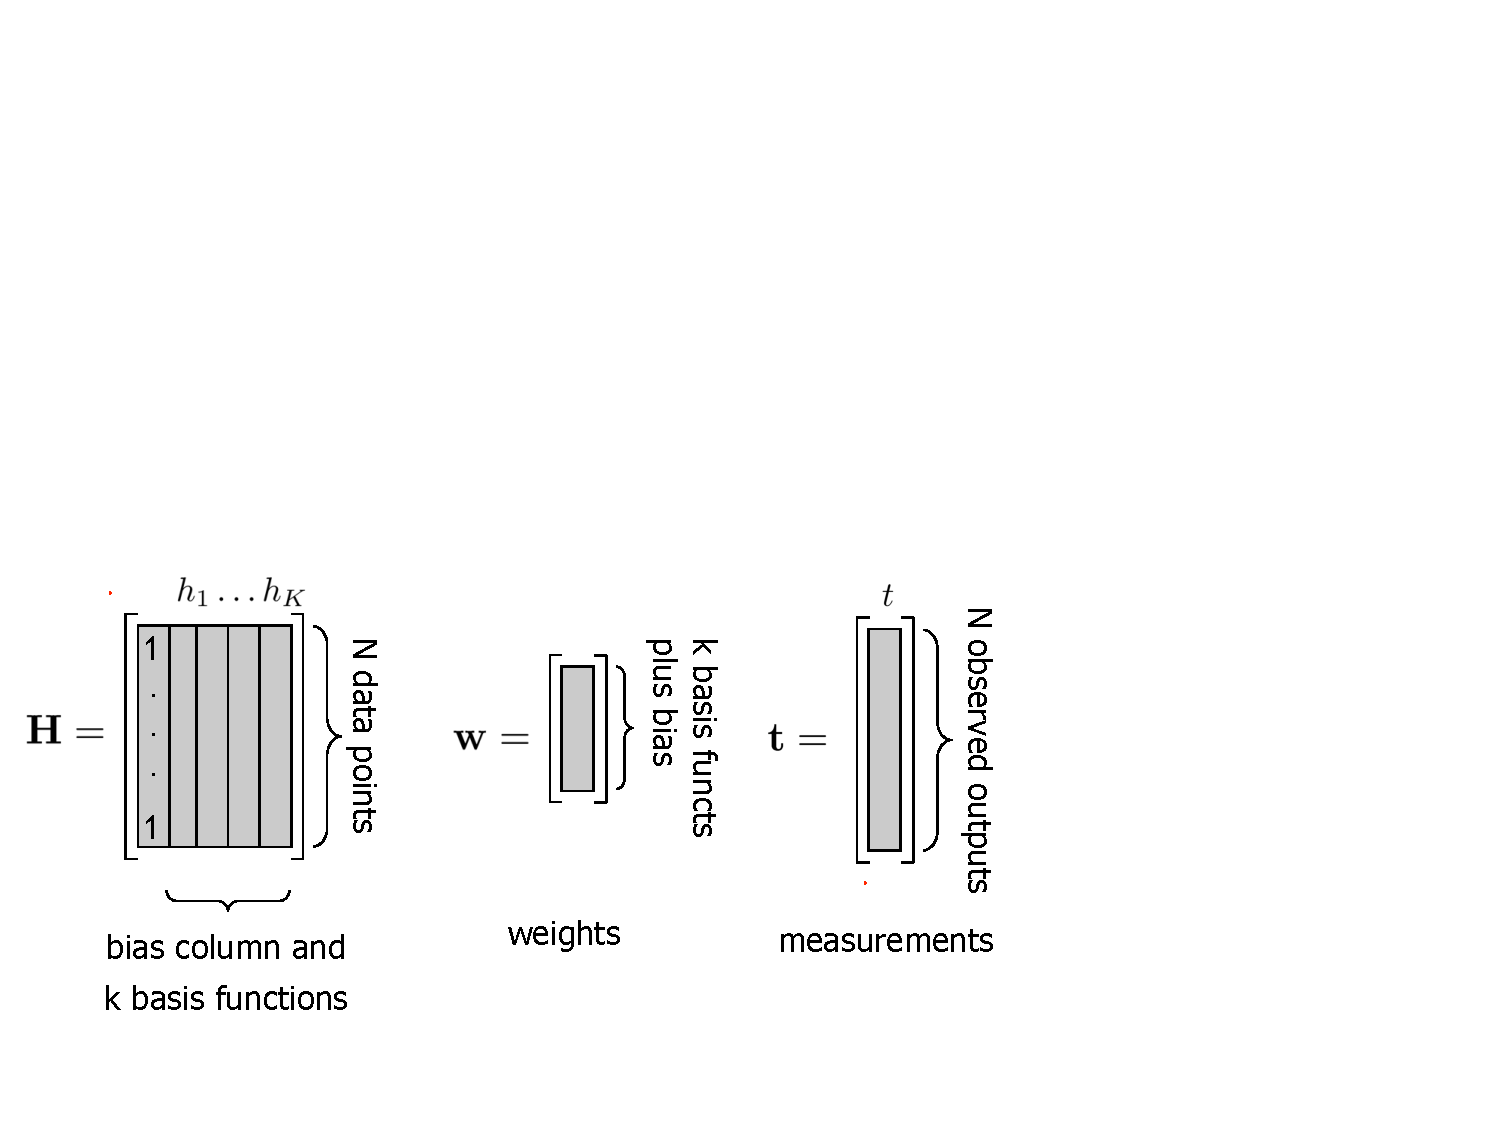
\includegraphics[width=3in]{figures/Least_squares_matricies.pdf}

\subsection{Regression: closed form solution}
 % derivation: http://courses.cs.washington.edu/courses/cse446/16wi/Slides/4_LinearRegression.pdf
\begin{align*}
	\bm{w}^* = \argmin_w (\bm{Hw} -\bm{t})^T (\bm{Hw} -\bm{t})  & \\
	\bm{F}(\bm{w}) =  \argmin_w (\bm{Hw} -\bm{t})^T (\bm{Hw} -\bm{t}) & \\
	\triangledown_{\bm{w}}\bm{F}(\bm{w}) = 0 \\
	2 \bm{H}^T (\bm{H}\bm{w}-\bm{t}) = 0  & \\
	(\bm{H}^T\bm{H}\bm{w}) - \bm{H}^T\bm{t} = 0 & \\
	\bm{w}^* = (\bm{H}^T\bm{H})^{-1}\bm{H}^T\bm{t} &
\end{align*}

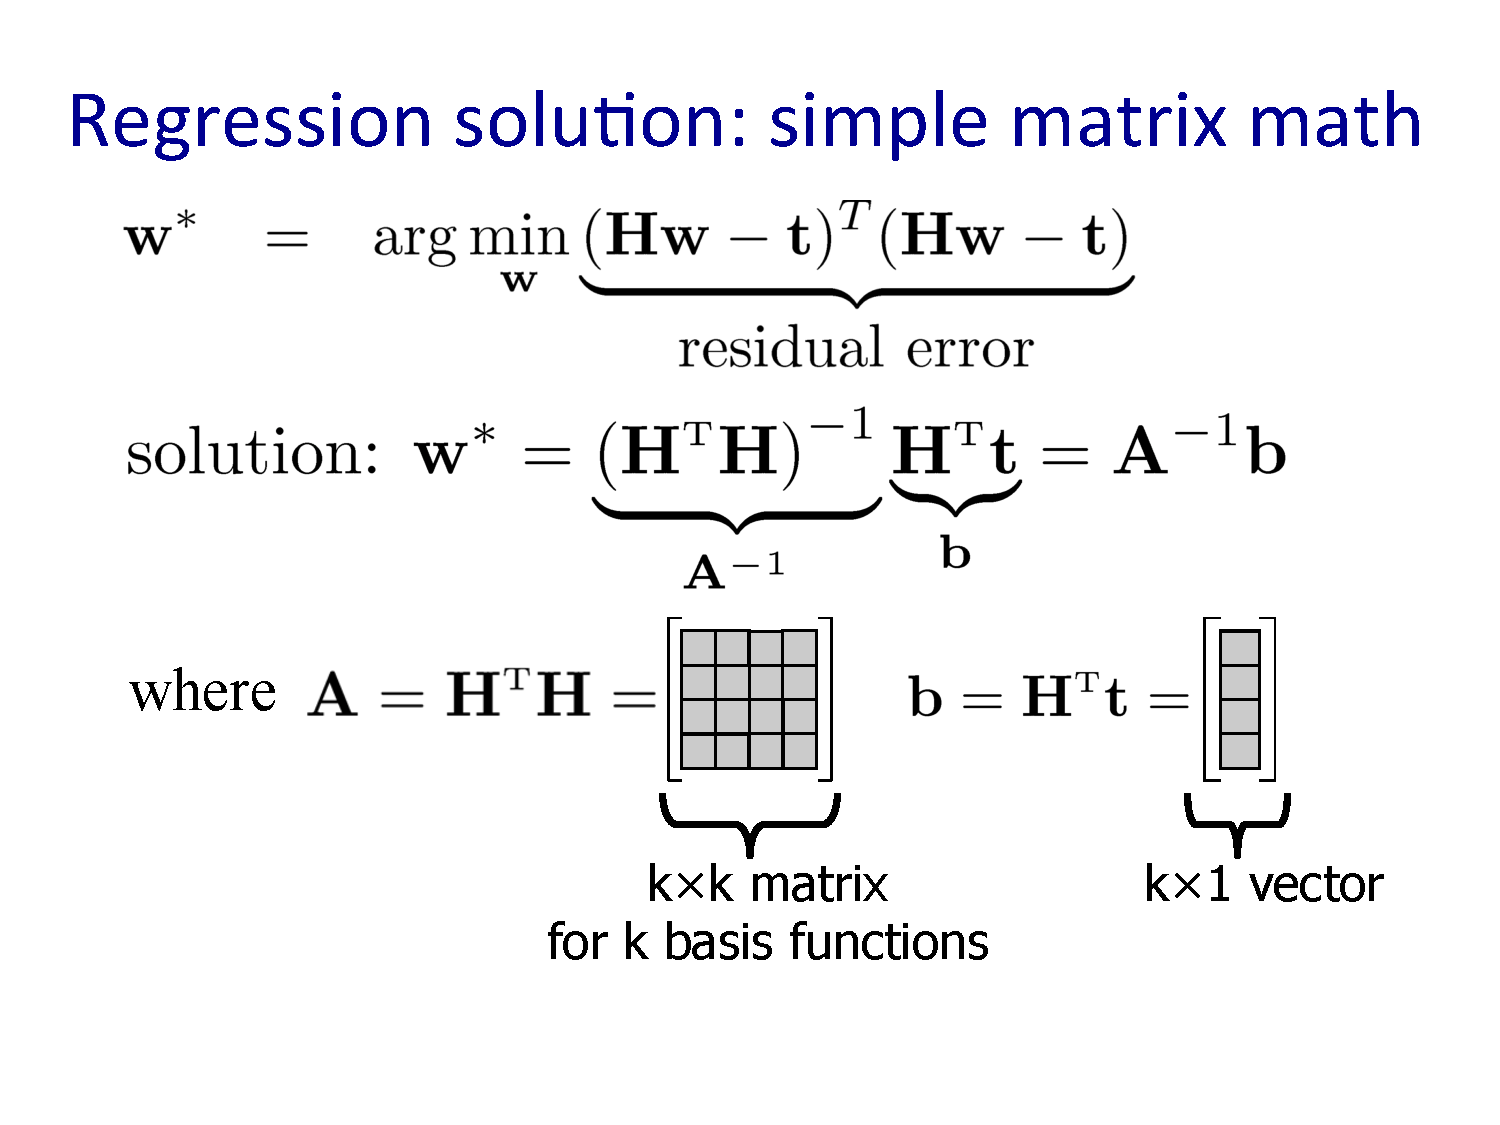
\includegraphics[width=3in]{figures/Regression_matrix_math.pdf}

Dimensions: 
\begin{itemize}
	\item $\bm{t}$:  N-dimensional  (N = \# of input data points) 
	\item $\bm{w}$: 
	\item $\bm{H}$: k + 1 by N.  N is \# of rows. 
\end{itemize}
\hfill \\

\subsubsection{Linear regression prediction is a linear function plus Gaussian noise}
%______TA e-mail 3/15________________________
\underline{Casual explanation:} \hfill \\
If we assume that our data $y_i$ is drawn from a linear function with some zero-mean Gaussian noise, i.e.

$$y_i = \sum_j w_j X_ij + \epsilon_i$$
(where $\epsilon_i$ is zero-mean gaussian noise drawn from Normal(0, $\sigma$)

Then we can show that the MLE estimates of $w_j$ are exactly the optimal weights obtained by minimizing the SSE: $\sum_i (y_i - w^T X_i)^2$

(note that the variance $\sigma$ actually doesn't matter for the derivation, you can just assume it's some positive number). \hfill \\ %%
\hfill \\
%______________________________
\underline{More formal explanation:} \hfill \\
We can model as linear combination of basis functions + noise $\epsilon$.  
It's safe to assume epsilon comes from Gaussian distribution.  \hfill \\

$t(\bm{x}) = \sum_i w_i h_i(\bm{x}) + \epsilon $ \hfill \\
Note: no $\mu$ because we set it to zero.  \hfill \\

We can learn $\bf{w}$ using MLE: 
$P(t | x, w, \sigma) = \frac{1}{\sigma \sqrt{2 \pi}} e^\frac{-[t - \sum_i w_i h_i(x)]^2}{2 \sigma^2}$
Take the log and maximize with respect to w:  (maximizing log-likelihood with respect to w) \hfill \\
$\displaystyle \ln P(D | \bm{w}, \sigma) = \ln(\frac{1}{\sigma \sqrt{2 \pi}})^N \prod_{j=1}^N e^\frac{-[t_j - \sum_i w_i h_i(x_j)]^2}{2 \sigma^2}$ \hfill \\
Now find the w that maximizes this: \hfill \\
$\argmax_w \ln(\frac{1}{\sigma \sqrt{2 \pi}})^N + \sum_{j=1}^N \frac{-[t_j - \sum_i w_i h_i(x_j)]^2}{2 \sigma^2}$ \hfill \\
the first term isn't impacted by $w$ so  \hfill \\
$= \argmax_w  \sum_{j=1}^N \frac{-[t_j - \sum_i w_i h_i(x_j)]^2}{2 \sigma^2}$ \hfill \\
switch to $\argmin_w$ when we divide by -1.  The numerator is constant.:  \hfill \\
$= \argmin_w  [t_j - \sum_i w_i h_i(x_j)]^2 $ \hfill \\

\textbf{Least-squares Linear Regression is MLE for Gaussians!!!}  \hfill \\ \hfill \\

If you have a polynomial you are fitting, how many basis functions are there (??)  \hfill \\ % asked Wed 1/27


\subsection{OLS Protocol (incomplete)}  \hfill \\
\begin{enumerate}
	\item Chose your basis functions $h_i$.  (Requires expertise).  Can be nonlinear, e.g. $x_1^2, \sin(x)$, etc. 
		\begin {itemize}
			\item 
				The number of parameters is len(H) + 1 (bias).  
				E.g. for fitting a parabola (formula $y = ax^2 + bx + c$), 
				you have 3 parameters: weights for basis functions $x$, $x^2$, and bias. 
				Typically the \# of basis functions is $<$ the \# of features.
		\end {itemize}
	\item Chose a regularization method so your weights don't get too big.  (see below)
	\item Plug them in to regression to get the weights ($w_i$s).  (Form the sum (residual squared error + regularization) that you want to minimize, then minimize.)    
	\item Make sure your weights aren't too big. 
	
\end{enumerate}

\subsection{Regularization in Linear Regression}  \hfill \\
You need to regularize to prevent parameters from growing too large.  
Both of these were built from the same set of basis functions; the right one is clearly over-fit. \hfill \\
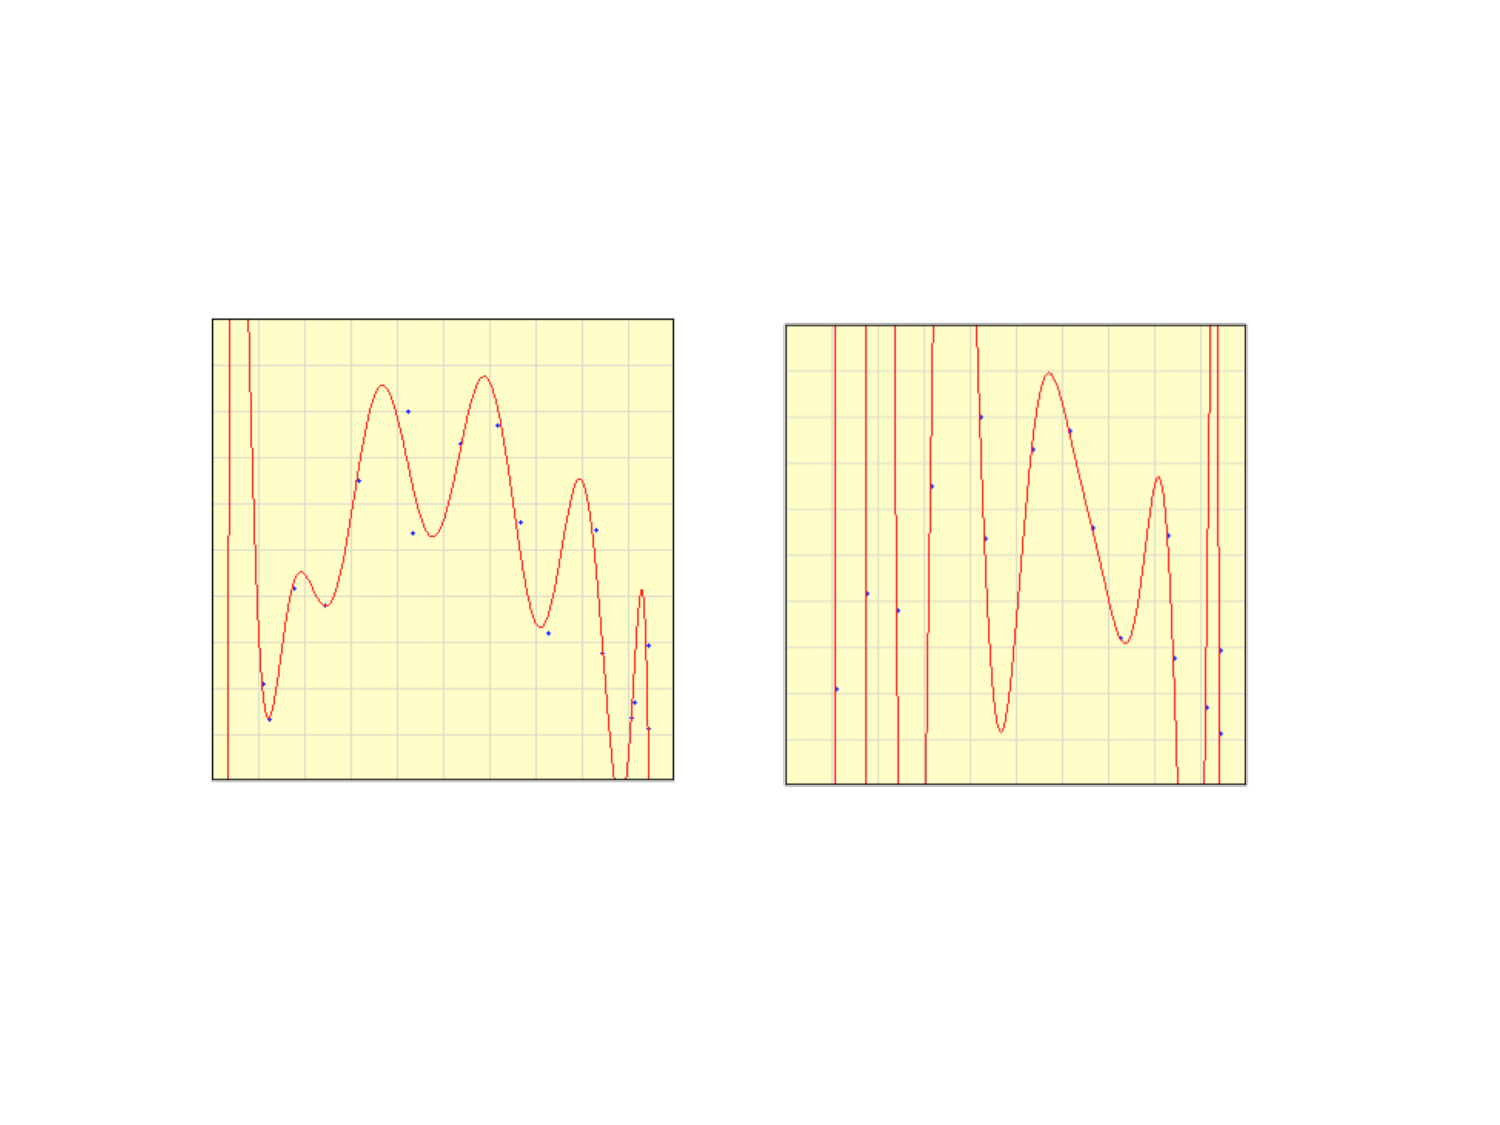
\includegraphics[width=1.2in]{figures/need_to_regularize.pdf}

\subsubsection{Ridge Regression}  \hfill \\
Ridge Regression is the most famous form of linear regression
Here is our old "ordinary" least squares objective function:   \hfill \\
$\displaystyle \widehat{w} = \argmin_w \sum_{j=1}^N [t(x_j) - (w_0 + \sum_{i=1}^k w_i h_i(x_j))]^2$   \hfill \\
It is the same as the previous ones but $i=0$ is pulled out.    \hfill \\
Now for ridge regression, we use that same notation.  \hfill \\
And we add a penalty term that isn't applied to the bias feature:
\begin{align*}
	\widehat{w}_{ridge} &= \argmin_w \sum_{j=1}^N [t(x_j) - (w_0 + \sum_{i=1}^k w_i h_i(x_j))]^2 + \lambda \sum_{i=1}^k w_i^2   \\
	&= \argmin_w (\bm{H}\bm{w} - \bm{t})^T(\bm{H}\bm{w}-\bm{t}) + \lambda \bm{w}^T I_{0+k} \bm{w}
\end{align*}
That $I_{0+k}$ matrix is this: 
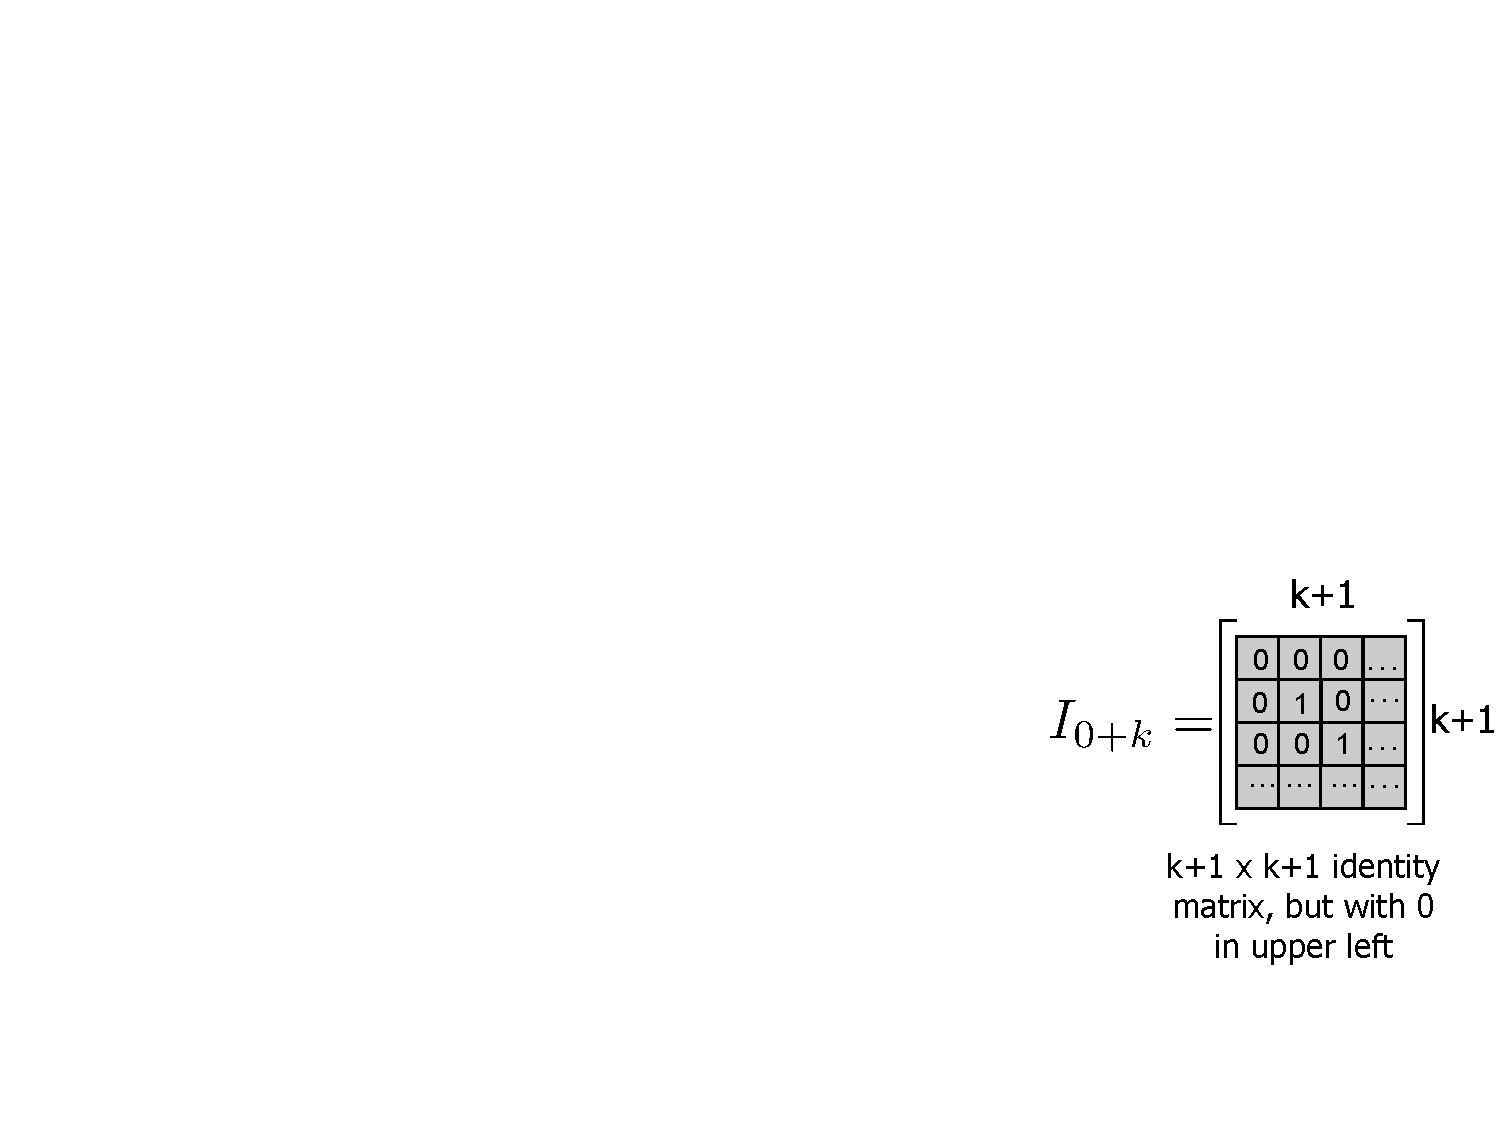
\includegraphics[width=1.0in]{figures/ridge_identity_matrix_with_zero.pdf}  \hfill \\
% Erick hasn't seen this notation.
Allows you to multiply the whole weight array without getting the bias term in there. 

Note: $W^TW$ is $w_i^2$ or $|| w_i ||^2$ 

A similar derivation leads to a closed form solution:  \hfill \\
% http://courses.cs.washington.edu/courses/cse446/16wi/Slides/4_LinearRegression.pdf 
$w_{ridge}^* = (\bm{H}^T\bm{H} + \lambda I_{0+k})^{-1}\bm{H}^T\bm{t}$ \hfill \\
(Recall that un-regularized regression was $w^* = (\bm{H}^T\bm{H})^{-1}\bm{H}^T\bm{t}$).  \hfill \\   \hfill \\

How do you chose how large $\lambda$ is? \hfill \\
* As $\lambda \rightarrow 0$, becomes same as MLE: unregularized.  Large magnitudes of coefficients. \hfill \\
* As $\lambda \rightarrow \infty$, all weights become 0.  \hfill \\   \hfill \\

\subsubsection{Experiment cycle}
\begin{enumerate}
	\item select a hypothesis $f$ to best match the training set.  
		(??) Is this the same as choosing your basis functions (?)
	\item isolate a held-out data set if you have enough data, or do K-fold cross-validation if not enough data. 
	\begin{itemize}
		\item tune hyperparameters ($\lambda$) on the held-out set or via cross-validation.  
			(Try many values of $\lambda$ and chose the best one.) 
		\item You can use the same held-out data set each time if that set is big.  
		\item If doing K-fold, divide the data into k subsets.  
				Repeatedly train on k-1 and test on the remaining one.  
				Average the results. 
		\item find the $w$ that minimizes the error.  
			(Do so by taking the derivative and setting = 0); 
			see ridge regression notes. 
	\end{itemize}
	\item Select basis functions
\end{enumerate}

\subsection{Regularization options: Ridge \& Lasso}  \hfill \\
Ridge: 
\begin{itemize}
	\item $ \displaystyle \widehat{w}_{ridge} = \argmin_w \sum_{j=1}^N [t(x_j) - (w_0 + \sum_{i=1}^k w_i h_i(x_j))]^2 + \lambda \sum_{i=1}^k w_i^2   $ 
	\item $L_2$ penalty.  ("$L_2$ norm of $\bm{w}$).  
		Large distances get penalized more.  $Y = x^2$: 
		don't want errors to cancel each other; differentiable. 
\end{itemize}
Lasso: \hfill \\
\begin{itemize}
	\item$ \displaystyle \widehat{w}_{ridge} = \argmin_w \sum_{j=1}^N [t(x_j) - (w_0 + \sum_{i=1}^k w_i h_i(x_j))]^2 + \lambda \sum_{i=1}^k |w_i|   $ 
	\item L1 penalty: linear penalty pushes more weights to zero.  Allows for a type of feature selection.  But it is not differentiable and there is no closed form solution. 
	\item L1 is absolute value: don't need to square it. 
	\item Lasso may be more useful when you have too many features for the amount of data you get.  
		Example: 100k parameters about companies to predict stock prices but only 100 data points.  
		Could tune lambda until you have about 100 nonzero weights. 
\end{itemize}

Your chose of penalty has huge effects on the algorithm! \hfill \\
Sometimes $L_1$ will do better than $L_2$ and vice versa, but usually $L_2$ is more powerful than $L_1$. \hfill \\
Would be better to use a combination of the penalties than to first reduce the number of features with $L_2$ before applying $L_1$.    \hfill \\
You can generate a lot of basis functions and use $L_1$ to chose the good ones. \hfill \\
\hfill \\

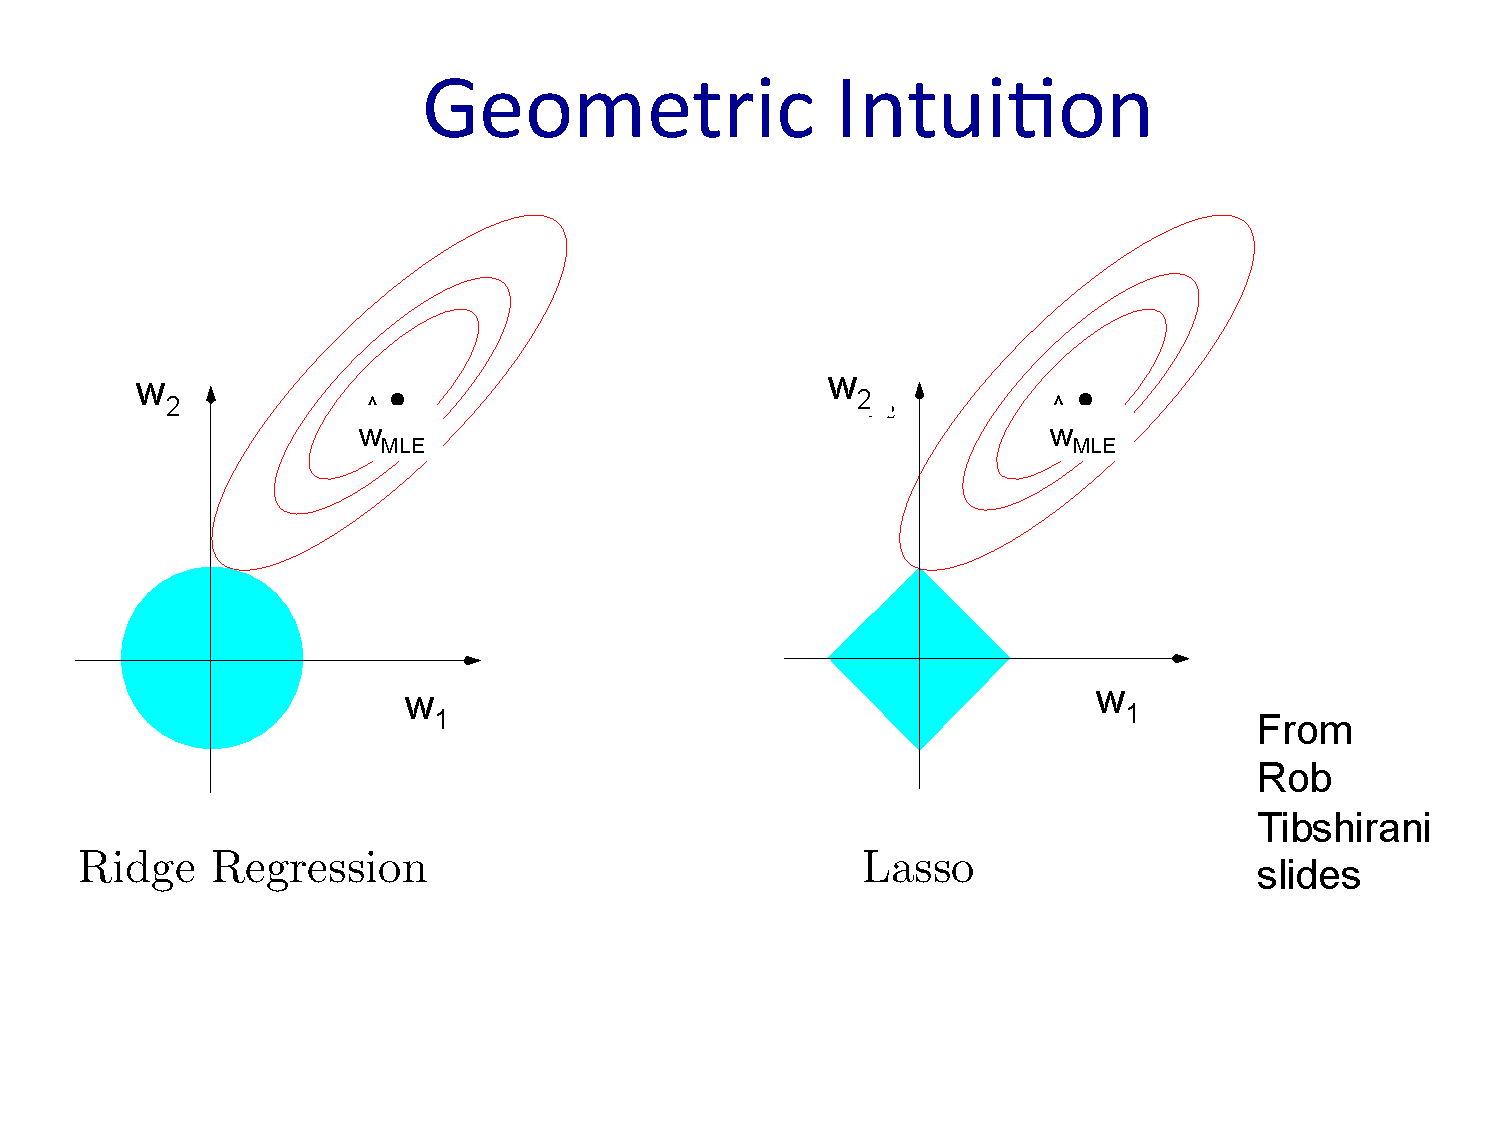
\includegraphics[width=3in]{figures/lasso_and_ridge_geometry.pdf}

This figure shows: 
\begin{itemize}
	\item The contour lines represent the maximum likelihood of the vector of weights.  
		All points on the contour have equal likelihood.
	\item The two axes represent different parameters for two of the weights.  (regression coefficients)
	\item Circles are characteristic of ridge regression (with L2 penalty): Penalty = the magnitude of the vector.
	\item Shapes that are pointy on the axes are characteristic of Lasso (with L1 penalty): the vector components get added. 
	\item Where the likelihood function touches in this $w_1, w_2$ space represents the coefficients of the weights.
		For Ridge Regression, we see that small but nonzero values of the coefficients can be obtained.
		For Lasso Regression, the curves are most likely to touch the diamond on the axes, 
		resulting in coefficients that are truly zero. 
\end{itemize} 

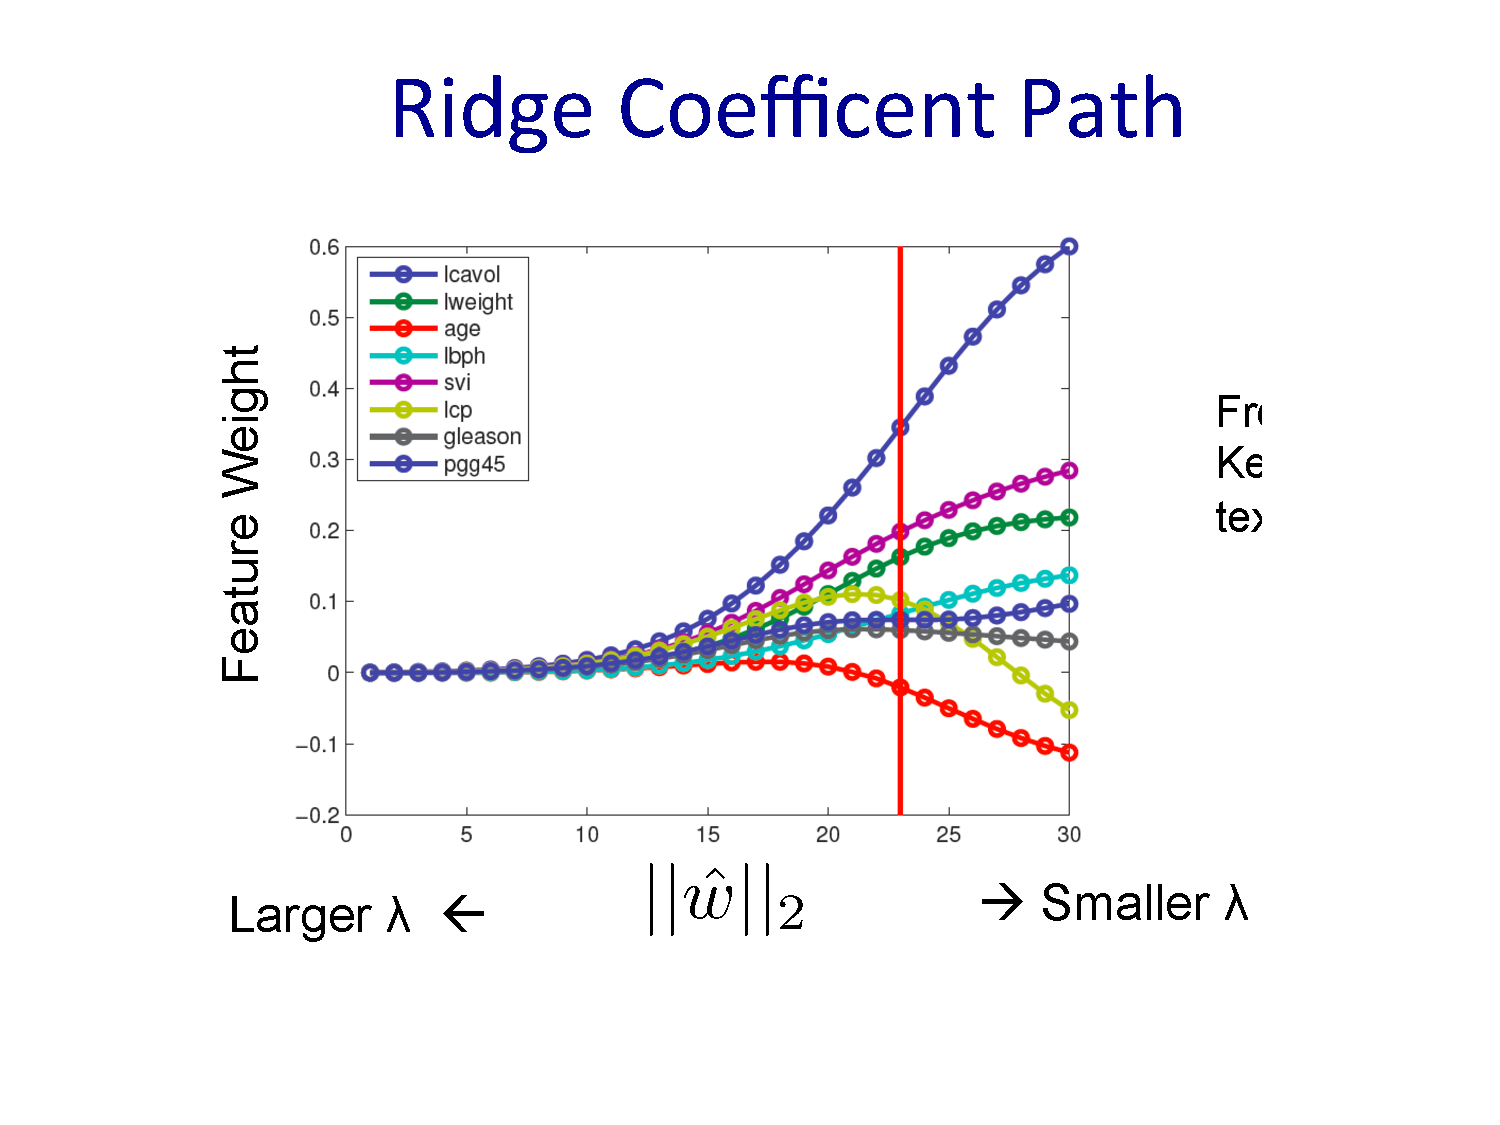
\includegraphics[width=1.8in]{figures/lambda_with_w2.pdf}  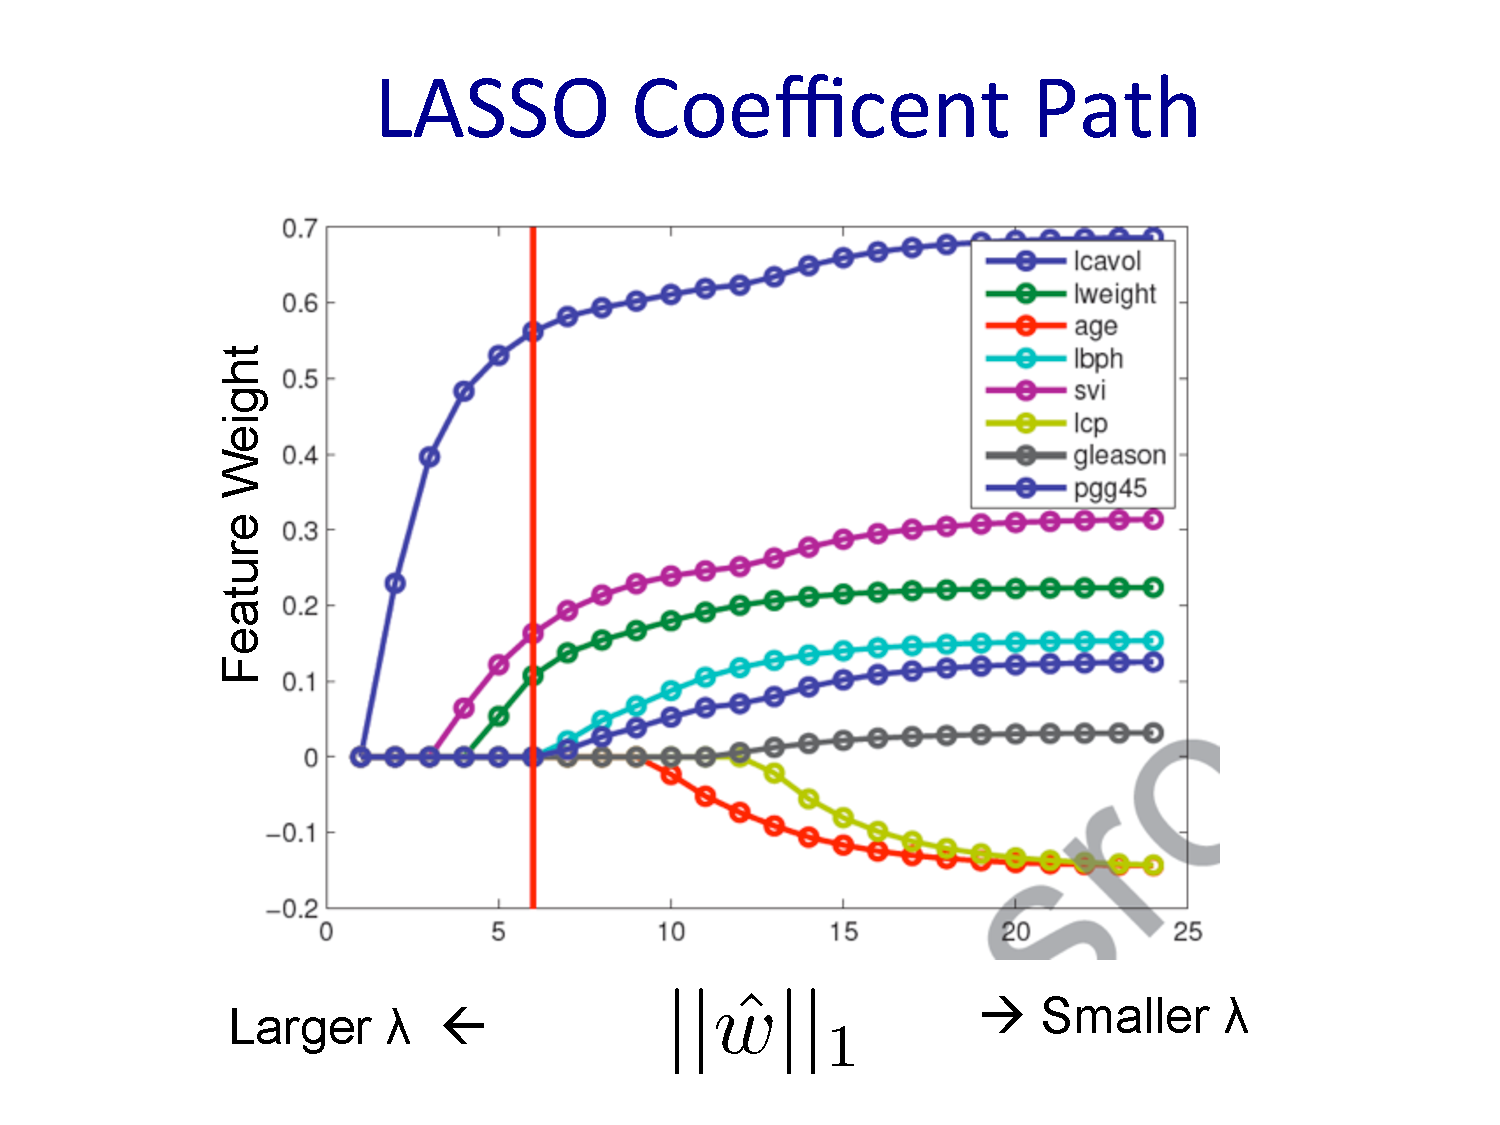
\includegraphics[width=1.6in]{figures/lambda_with_w1.pdf}
Don't compare coefficient magnitudes at given $\lambda$s, 
but do note that for Ridge the gradually come away from the zero axis and in Lasso they are zero until they pop out.   \hfill \\ \hfill \\

\subsection{Bias-Variance Tradeoff}
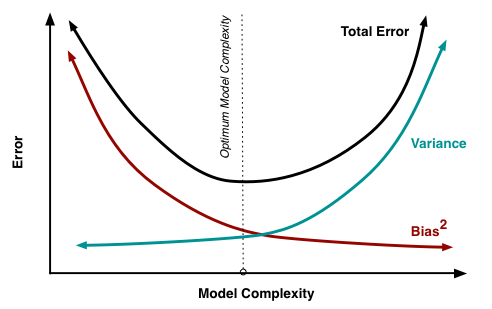
\includegraphics[width=2.0in]{figures/biasvariance.png} 

Your choice of hypothesis class (e.g. degree of polynomial) introduces learning bias.  \hfill \\
The more complex the model, the more the \_\_\_\_ set accuracy goes down  \hfill \\  % had "training" with ?
\textbf{A more complex class } $\rightarrow$ less bias and more variance.   \hfill \\ \hfill \\

From https://www.youtube.com/watch?v=Rm6s6gmLTdg: hfill \\
High bias = inability to represent the true function in the class of functions we are willing to tolerate.
Pulls us to a particular function or class of functions regardless of the data.
Can be from looking only at a specific type of function, or by having strong regularization  \hfill \\
High variance = extremely dependent on the exact data they were trained on.
Might fit the data well, but may do poorly on a different data self.  \hfill \\


From Wikipedia: \hfill \\  % https://en.wikipedia.org/wiki/Bias%E2%80%93variance_tradeoff
Ideally, one wants to choose a model that both accurately captures the regularities in its training data, 
but also generalizes well to unseen data. Unfortunately, it is typically impossible to do both simultaneously. 
High-variance learning methods may be able to represent their training set well, but are at risk of overfitting 
to noisy or unrepresentative training data. 
In contrast, algorithms with high bias typically produce simpler models that don't tend to overfit, 
but may underfit their training data, failing to capture important regularities. \hfill \\  \hfill \\

Models with low bias are usually more complex (e.g. higher-order regression polynomials), 
enabling them to represent the training set more accurately. 
In the process, however, they may also represent a large noise component in the training set, 
making their predictions less accurate - despite their added complexity. 
In contrast, models with higher bias tend to be relatively simple (low-order or even linear regression polynomials), 
but may produce lower variance predictions when applied beyond the training set. \hfill \\ \hfill \\

Adding features (predictors) tends to decrease bias, at the expense of introducing additional variance.   \hfill \\
\hfill \\

Solutions:
\begin{itemize}
	\item Dimensionality reduction and feature selection can decrease variance by simplifying models. 
	\item Similarly, a larger training set tends to decrease variance. 
	\item Use tunable modeling parameters such as applying more significant regularization.
\end{itemize}

\textbf{If held-out is too small, we can end up over-fitting.}


\hfill \\  \hfill \\

\subsection{Error Definitions}

\underline{True ("Prediction") Error}:   \hfill \\
Since the training set error can be a poor measure of the "quality" of the solution, we can use prediction error ("true error").  
The error over all possibilities.   Instead of sum, take expectation. 
\begin{align*}
	error_{true}(\bm{w}) &= E_X[(t(\bm{x_j})-\sum_{i} w_i h_i(\bm{x_j}))^2] \\
		& \mbox{Gold Standard:} \\
	error_{true}(\bm{w}) &= \int_x (t(\bm{x_j})-\sum_{i} w_i h_i(\bm{x_j}))^2 p(\bm{x}) d\bm{x}
\end{align*}

% TA 3/15/2016:
$p(x)$ is assumed to be the "true" distribution of the data, which we don't actually know. 

How to get $p(\bm{x})$?  Need to know the true distribution of the data (?).  
You almost never know how to compute $p(x)$.
And, the integral is a very big sum. \hfill \\  \hfill \\

% Find $p(x)$ using monte-carlo integration. \hfill \\

% TA 3/15/2016:
To do this, you need to split your data into training and test set. 
If we have a dataset which is randomly sampled from $p(x)$, which we assume our data is, we can estimate the true error using the average of the samples. 
Since we train on our training set, the error might be a bad estimate of the true error (we're biased to decrease the error), so we use a separate hold-out testing set to approximate the true error in instead.

Sample a set of i.i.d. points  $\{ \bm{x}_1, \dots, \bm{x}_M \}$ from $p(x)$.   \hfill \\
Approximate the integral with the sample average:
$$ error_{true}(\bm{w}) \approx \frac{1}{M} \sum_{j=1}^M \left( t(\bm{x}_j - \sum_i w_i h_i(\bm{x}_j) \right) $$
That is the sampling approximation of the predicted error: \hfill \\
That leads to a fair approximation.   \hfill \\

\hfill \\  \hfill \\

The true prediction error is the expectation over \textbf{future} test cases you don't have.  
Since you don't have the x values, you go to probability. 
Pick a point from the distribution, and calculate the \_\_\_\_\_.     \hfill \\  \hfill \\

Don't use the training data to predict true error; you've already trained to that data!  You would have too optimistic of a prediction for true error. 

Prediction error is high when the model is too simple \underline{and} too complex, unlike training set error which only penalizes too simple.  \hfill \\
\hfill \\

\underline{Training Set Error}:  \textbf{optimistically biased}  (a.k.a. training error) \hfill \\
$\displaystyle  error_{train}(\bm{w}) = \frac{1}{N_{train}} \sum_{j=1}^{N_{train}}(t(\bm{x_j})-\sum_{i} w_i h_i(\bm{x_j}))^2$ \hfill \\
Decreases exponentially with model complexity.   \hfill \\
\textbf{Training error is a poor prediction of prediction error!} \hfill \\
You expect to see training error to decrease with complexity, but that doesn't mean you have a good solution!  \hfill \\
\hfill \\  \hfill \\
% http://courses.cs.washington.edu/courses/cse446/16wi/Slides/4_LinearRegression.pdf


\underline{Test Error}: (our final measure)  \hfill \\
Uses the same formula as prediction error, except that we have never observed the test data.  See formula below. 
We expect the true error to be smile shaped if the x-axis is model-complexity. 
\hfill \\ \hfill \\

\underline{\textbf{Testing is for the user of your algorithm. }}
The user doesn't care about the values in your model.  They just care about how well it works.  
 They dont' care about the value of your hyperparameters. 


\subsubsection{Effects of $\lambda$ value on model}
% week 4 typed notes. 
 \begin{itemize}
 	\item high lambda $\rightarrow$ simple model $\rightarrow$ lots of zeros $\rightarrow$ high error. 
	\item with lambda = 0 $\rightarrow$ converges ridge regression to regular regression. 
	\item with enough traiing data and lambda = 0, we expect overfitting $\rightarrow$ small training error. 
\end{itemize}

\subsubsection{Choosing $\lambda$}
How to find lambdas? 
\begin{itemize}
	\item try a bunch and find which does best on the held out data set.  
		Can't touch test data, even w/ stick so use held-out set. 
	\item Do k-fold cross validation to pick the lambda that gives minimum error. \hfill \\
		Average over the loss curves Loss($fold_i$, $\lambda$) \hfill \\ 
		Minimum error = lowest loss on the hold-out set (the curve should look U shaped, so you just find the bottom of the U).  \hfill \\
		May not find the bottom-of-the-U shape lambda.    \hfill \\
		But it is ok to be off a bit; the red U might be pretty flat at the bottoms. \hfill \\
\end{itemize}		
This use of the held-out data doesn't count as training.  
Lambda is fixed each time, and we train separately. 
Training on training data, just watching the number on the held-out set. \hfill \\
\textbf{The model's parameters are not determined by the held-out data} \hfill \\
\hfill \\

How do you chose the range of lambda? (practical solution) 
\begin{itemize}
	\item You are limited to a grid search over values of lambda. 
	\item You need a strategy for sweeping that space.   
		Could do a "binary search", or something like a gradient search: 
		take a step until we screw it up, and step back smaller.   
		If it gets worse, you take a smaller step.
	\item From your loss, take the value of your loss (compute it).  \hfill \\
		Loss = $(t(x) - \sum w_i h(x_i))^2$  
        		\textbf{"You should be able to find loss given w}
            	Can compute norm of W, too.  
		If your loss is on the order of 1000 and your norm is on the order of 1, you can use these for defining search space.
                	Firs try lamba = 1, 10, 100, 1000.  
		Find the best from there then explore around there.
		If 100 was good, try 200, etc.   
		You just want to know in which order the loss function is going to appear. 
\end{itemize}

\subsubsection{How to handle error calculations:}
Given a dataset, randomly split it into two parts:  \hfill \\
* training data: $\{ \bm{x_1}, \dots, \bm{x_{N_train}} \}$   \hfill \\
* test data: $\{ \bm{x_1}, \dots, \bm{x_{N_test}} \}$   \hfill \\
Use the training data to optimize parameters $\bm{w}$. \hfill \\
To calculate the test set error, you use the final solution $\bm{w^*}$ and calculate \hfill \\
$\displaystyle error_{test}(\bm{w}) \approx \frac{1}{N_{test}} \sum_{j=1}^{N_{test}} (t(\bm{x_j} - \sum_i w_i h_i(\bm{x_j}))^2$  \hfill \\

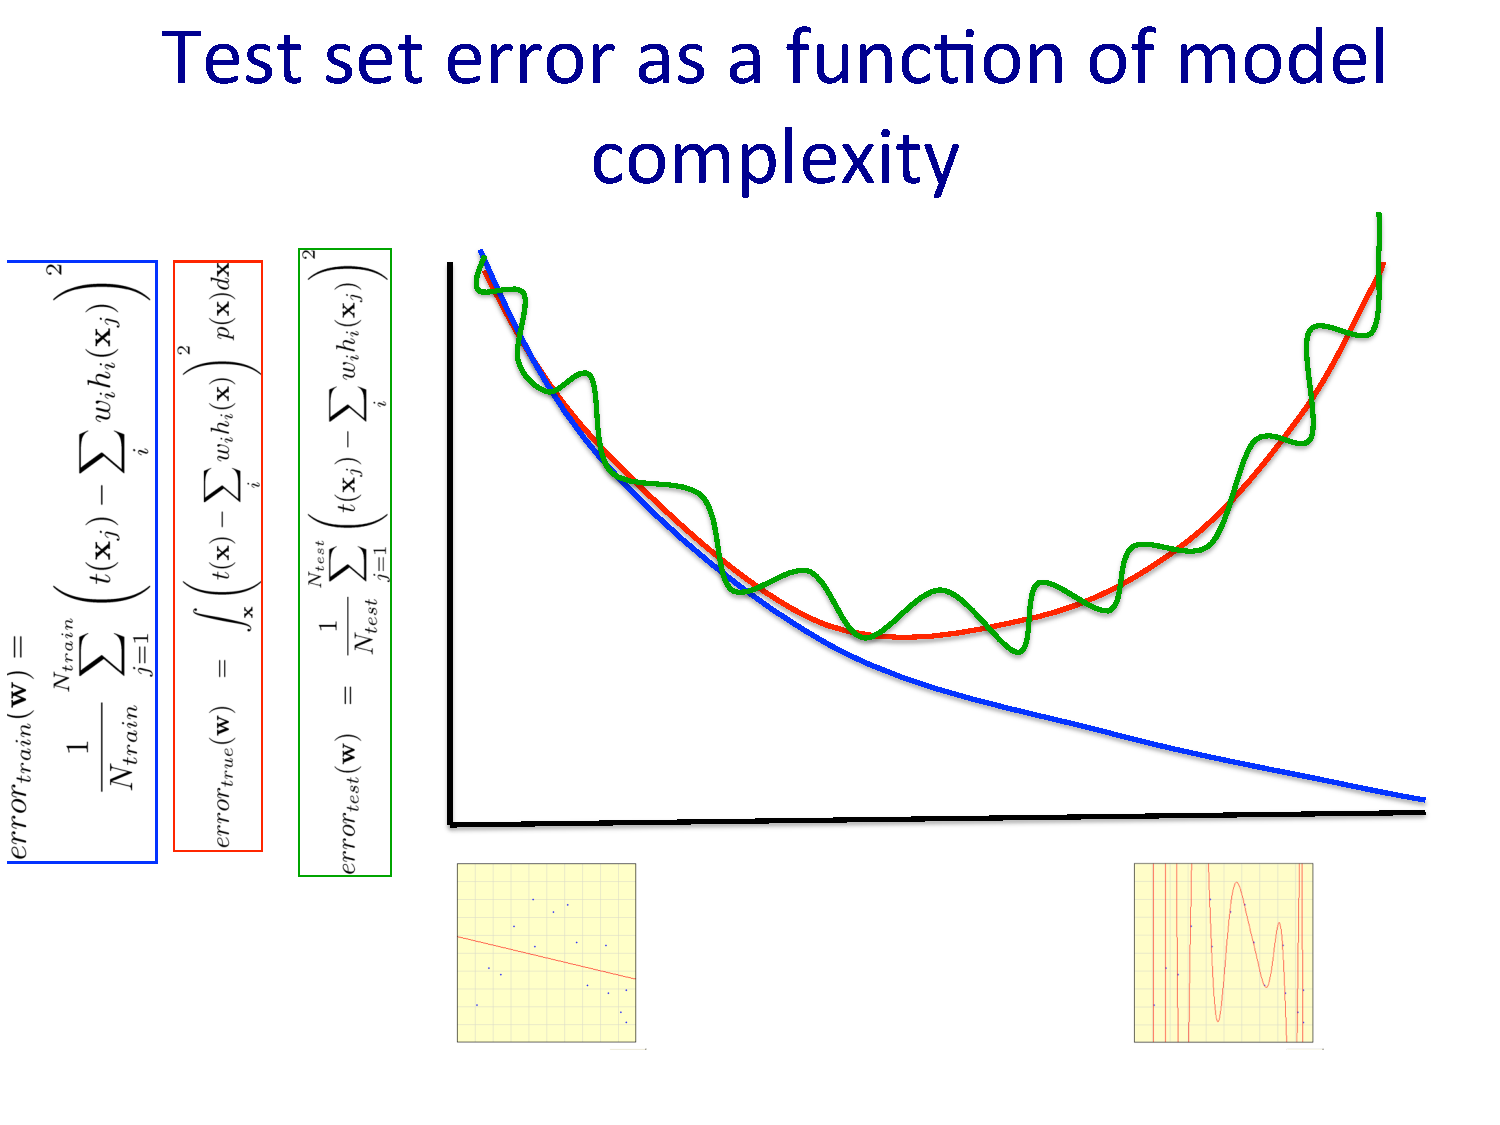
\includegraphics[width=3in]{figures/errors_as_f_of_complexity.pdf}   \hfill \\
(blue is train, red is true, green is test) \hfill \\

\subsubsection{overfitting}
Assume: \hfill \\
* Data generated from distribution D(X,Y). \hfill \\
* A hypothesis space H \hfill \\
Define:  \hfill \\
* Training error: $error_{train}(h)$ \hfill \\
* Data (true) error: $error_{true}(h)$ \hfill \\
We say $h$ \textbf{overfits} the training data if there exists an $h' \in H$ such that:  \hfill \\ 
* $error_{train}(h) < error_{train}(h)'$ and $error_{true}(h) > error_{true}(h)'$

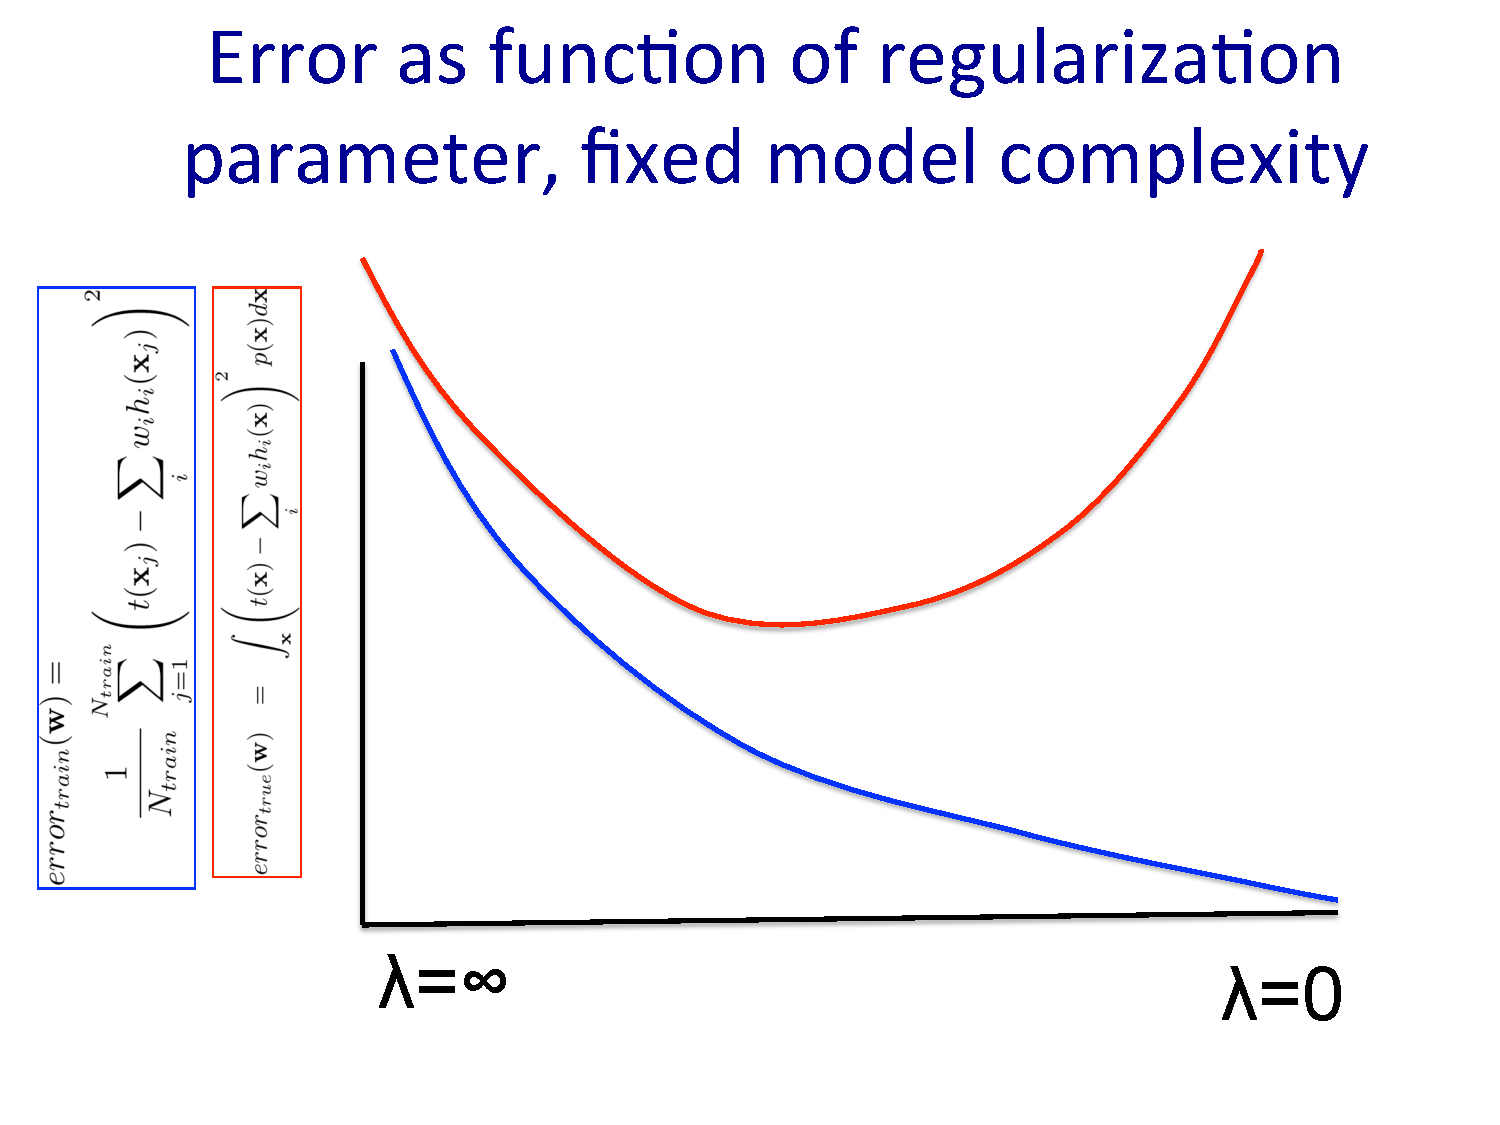
\includegraphics[width=2in]{figures/Error--vs_lambda--fixed_model_complexity.pdf}   \hfill \\
Lambda (the regularization parameter) is fixed.  Blue = training set error.  
Leads to overfitting/too-large-parameters when $\lambda$ --> 0. 
Red = true error, which likes a happy medium $\lambda$.  \hfill \\  \hfill \\

\textbf{Warning}: your test set is only unbiased if you never ever ever do \textbf{any} learning on the data. 
This includes using the test data to select for the degree of the polynomial you fit.   \hfill \\  \hfill \\
(Recall, you can create a held-out/validation set from your training data or do k-fold validation.)  \hfill \\
\hfill \\

The height of the true error (red curve) is the "bias".  \hfill \\

\subsubsection{What you need to know}
Regression:
\begin{itemize}
	\item Basis functions = features
	\item Optimizing a sum of squared errors
	\item Relationship between regression and Gaussians
\end{itemize}
Regularization
\begin{itemize}
	\item Ridge regression math
	\item LASSO formulation
	\item How to set lambda
\end{itemize}
Bias-Variance trade-off







\section{General Vocab}
\smallskip \hrule height 2pt \smallskip
 
 \begin{itemize}
 	\item \textbf{classification} - ??? Finding a f that converts X to Y where Y are categorical.  (Not regression).  
	\item \textbf{supervised learning} - at training time we are given a set of features with discrete class labels.  % Wk 4 audio transcription.
 	\item \textbf{held-out data}: 
			the terms "held-out" and "validation" are usually synonymous  % 2/25/2015 class forum (my question)
	\item \textbf{hypothesis space}: ?  E.g. binomial distribution for coin flip.  	
 	\item \textbf{prediction error}: measure of fit (?) 
	\item \textbf{regularization}: a process of introducing additional information in order to solve an ill-posed problem or to prevent overfitting  % https://en.wikipedia.org/wiki/Regularization_(mathematics)
	\item \textbf {norm}.  A scalar (not vector!) measure of distance between two vectors.  % E confirmed 3/6/2016
					You can divide by this scalar to \underline{norm}alize, but that is just one use case.
					You can also use either norm as a regularization term. 
	\item \textbf{L1} norm.  Just add the absolute values of the components.  % E confirmed 3/6/2016
	\item \textbf{L2} norm.  Can be used to regularize, or to normalizing features. 
		\begin{itemize}
			\item Euclidean vector length.  Pythagoras style. 
			\item You can do $l_2$ normalization for a feature vector to get a unit vector: 
				Convert $x$ to $\hat{x}$ so that if you form $||\hat{x}||_2^2 = 1$
				Can also do $l_1$
		\end{itemize}
	\item \textbf{L2} distance:  Pythagoras distance between two vectors. 
	\item \textbf{convergence} - if you add more data and you don't get different parameters, the model has converged. 
	\item \textbf{kernel}: some transformation of your features that improves your classification %Erick 1/30/2015
	%\item \textbf{}
	\item \textbf{affine}: indicates that the subspace need not pass through the origin.  % Intro to statistical learning Ch 9.1
	\item \textbf{support vector}: data points that �support� the maximal margin hyperplane in the sense that if these points were 				moved slightly then the maximal margin hyper- plane would move as well.   % Intro to statistical learning Ch 9.1
	\item \textbf{marginal likelihood}: 
	\item \textbf{marginalized out} = integrated out % https://en.wikipedia.org/wiki/Marginal_likelihood

 \end{itemize}
 
 Concepts:
\textbf{likelihood vs posterior}: \hfill \\

	likelihood*prior = constant*posterior.  $P(Y|X)$ is likelihood, $P(X|Y)$ is posterior.  
\hfill \\
\hfill \\

\subsubsection{Normalizing data}
Options:
\begin{itemize}
	\item min/max
	\item sigmoid
	\item $L_1$ norm
	\item $L_2$ norm
\end{itemize}
Note $L_1$/$L_2$ normalization versus penalty/regularization!!  

\subsubsection{Size for modeling P$(Y=y | X)$}
		How many parameters are needed to model $P(y | x_1, x_2, ..., x_d)$?  
		Assume Y is discrete and all the $x_i$ are binary.
		You have d binary features, so you have $2^d$ probabilities in order to classify every possible input.   % Erick
		
		The number of parameters in the PDF of $P(Y=y | X)$ is $2^d$ (+ 1 for bias sometimes).  
		The size (\# of nodes??) of the conditional probability tree grows exponentially.
		% The tree is the tree of conditional probabilities, i'll bet  % Erick. 
		The data is just a table with Y and X columns.  
		
		We only need $2^d$ (or perhaps $2^{(d+1)}$) to get all possibilities specified.  
            	If each feature can take m values instead then we have $m^d$.  Not binary any more!
		The number of parameters can get very big but Naive Bayes can handle it.  \hfill \\
		
		What is the order of the size of the parameters you need to do the full conditional probability?
		For Naive Bayes it is d; \textbf{linear}.  And the full conditional would be exponential! 

\subsubsection{Maximum Likelihood Estimation (MLE)}

\textbf{Take log, take derivative, set equal to zero.} \hfill \\

Memorize. Likelihood is DATA. \hfill \\  % e-mail to self 2/1/2015 

The best mu for a gaussian is the mean. 
Maximized probability of this data being produced by the distribution. 
The data is most likely to be generated if the mean is mu. 
Did same for sigma.  We realized best way is to use the variance.  \hfill \\

\textbf{Wikipedia:}

To use the method of maximum likelihood, one first specifies the joint density function for all observations. For an independent and identically distributed sample, this joint density function is:

$$  f(x_1,x_2,\ldots,x_n\mid\theta) = f(x_1\mid \theta)\times f(x_2|\theta) \times \cdots \times  f(x_n\mid \theta). $$
  
Now we look at this function from a different perspective by considering the observed values $x1, x2, \dots, xn$ to be fixed "parameters" of this function, whereas ? will be the function's variable and allowed to vary freely; this function will be called the likelihood:


 $$  \mathcal{L}(\theta\,;\,x_1,\ldots,x_n) = f(x_1,x_2,\ldots,x_n\mid\theta) = \prod_{i=1}^n f(x_i\mid\theta) $$
  
Note that " ; " denotes a separation between the two input arguments: $\theta$ and the observations $x_1,\ldots, x_n$.

In practice it is often more convenient to work with the logarithm of the likelihood function, called the log-likelihood:


   $$ \ln\mathcal{L}(\theta\,;\,x_1,\ldots,x_n) = \sum_{i=1}^n \ln f(x_i\mid\theta) $$
  
or the average log-likelihood:

  $$ \hat\ell = \frac1n \ln\mathcal{L} $$
  
The hat over $\ell$ indicates that it is akin to some estimator. Indeed, $\hat{\ell}$ estimates the expected log-likelihood of a single observation in the model.

The method of maximum likelihood estimates $\theta_0$ by finding a value of $\theta$ that maximizes $\hat\ell(\theta;x)$. This method of estimation defines a maximum-likelihood estimator (MLE) of $\theta_0$:


    $$  \{ \hat\theta_\mathrm{mle}\} \subseteq \{ \underset{\theta\in\Theta}{\operatorname{arg\,max}}\ \hat\ell(\theta\,;\,x_1,\ldots,x_n) \} $$

	
\subsubsection{MLE vs MAP}
\begin{itemize}
		\item both MLE and MAP are point estimates.  No estimate of uncertainty.  % https://www.youtube.com/watch?
		\item MLE fits a probabilistic model $P(x | \theta)$ to data to estimate $\theta$. % http://www.cs.colostate.edu/~cs545/fall13/dokuwiki/lib/exe/fetch.php?media=wiki%3A13_naive_bayes.pdf
			You chose the parameters $\theta$ that maximize $\ln P(X | \theta)$
		\item MLE is more likely to overfit; MAP regularizes to prevent overfitting.  \hfill \\  % https://www.youtube.com/watch?v=kkhdIriddSI 
		\item MAP doesn't have all the nice asymptotic relationship, but tends to look like MLE asymptotically.
			As your data goes to infinity, your prior foes to the data.  % https://www.youtube.com/watch?v=kkhdIriddSI 
		\item unlike MLE, MAP is not invariant under reparameterization.  (A disadvantage)  % https://www.youtube.com/watch?v=kkhdIriddSI
		\item in MAP, you have to chose a prior.  Sometimes not fun to pick.  % https://www.youtube.com/watch?v=kkhdIriddSI
\end{itemize}

\subsubsection{How Naive Bayes, MLE, and MAP fit together}  % Erick approved.
In order to do Bayesian inference, you put your likelihood into Bayes rule.  That has nothing to do with Naive Bayes.
If you just maximize the ML equation, that gives you MLE.
If you maximize the posterior that you get from Bayes rule then you have MAP.  
All that is true across analysis.

A full Bayesian analysis for many classification problems is too hard.  Too parameter rich, too computationally expensive.
You can simplify by making the Naive Bayes assumption. 
In machine learning world you will usually do this simplification. 

Note: Erick doesn't think he will ever use Naive Bayes.  
He does statistical analysis, not Naive Bayes.  
Naive Bayes is a much smaller and specialized thing than general Bayesian analysis.
That's the statistician perspective. 

For ML, it is a nice way of gettitng regularized estimates. 
You could also use Bayes to relate parameters in a model. 
That's what Erick does a lot. 

\subsubsection{Smoothing}
Can reduce sensitivity to zero values when multiplying probabilities.
\begin{itemize}
	\item prior distribution for binaries: Beta distribution. 
	\item Laplace smoothing for multinomial. 
	
\textbf{Bayes b/c you aren't going to see a feature vector that matches one in training.}
	We are \textbf{not} going to see a feature that is the exact same as a feature in the training set. 
	That's \textbf{why} we estimate w/ Bayes.   % week 5 notes
\end{itemize}

\subsubsection{Generate vs. Discriminative}
logistic: discriminative  \hfill \\
Naive Bayes:  generative   \hfill \\
\hfill \\

One can only distinct between whether it is something, the other can say how likely. \hfill \\

Two big categories of approaches for ML: \hfill \\
\underline{Generative}:
		Those that try to estimate the joint distributions between labels and features/data. 
		Model the joint distributions. $P(X,Y) = f(X|Y) P(Y) or P(Y|X)f(x)$.  
		"Class conditional densities" are modeled.  % https://www.youtube.com/watch?v=oTtow2Ui8vg 
		\textbf{If you can create a distribution, you can sample from it.}  % wk 5 transcript
		More powerful if you have enough data to estimate the densities, but worse without enough data.
		Natural interpretation.  
		Bayes classification is an example.    
		Naive Bayes is one that can produce p(Data,Zebra), except you've made a lot of assumptions.   \hfill \\  % Wed Wk 5 transcript
		P(Data,Zebra) is a pdf over samples. 
		If you didn't relax all the constraints when going from Bayes to Naive Bayes, you could paint a zebra.   \hfill \\
		A joint probability model with evidence variable.   \hfill \\  % Lec 7: preceptrons
 \hfill \\
\underline{Discriminative}:
		No generative model, no Bayes rule, often no probabilities at all!   \hfill \\  % Preceprtons (Lec 7)
		Those that directly estimate the decision boundary.  "discriminative decision boundary".  Find $P(Y|X)$ \hfill \\
		Describing how to generate random instances X conditioned on the target attribute Y.  \hfill \\
		The discriminative classifier is like a lazy painter.  \hfill \\  % Wed Wk 5 transcript
		You can get decision boundary out of a generative model but it is over-kill if you only want to produce a label.  \hfill \\  % Wed Wk 5 transcript
		 85\% of time discriminative outperforms.  B/c p(Data,Zebra) is hard to estimate.  \hfill \\  % Wed Wk 5 transcript
		 
		 
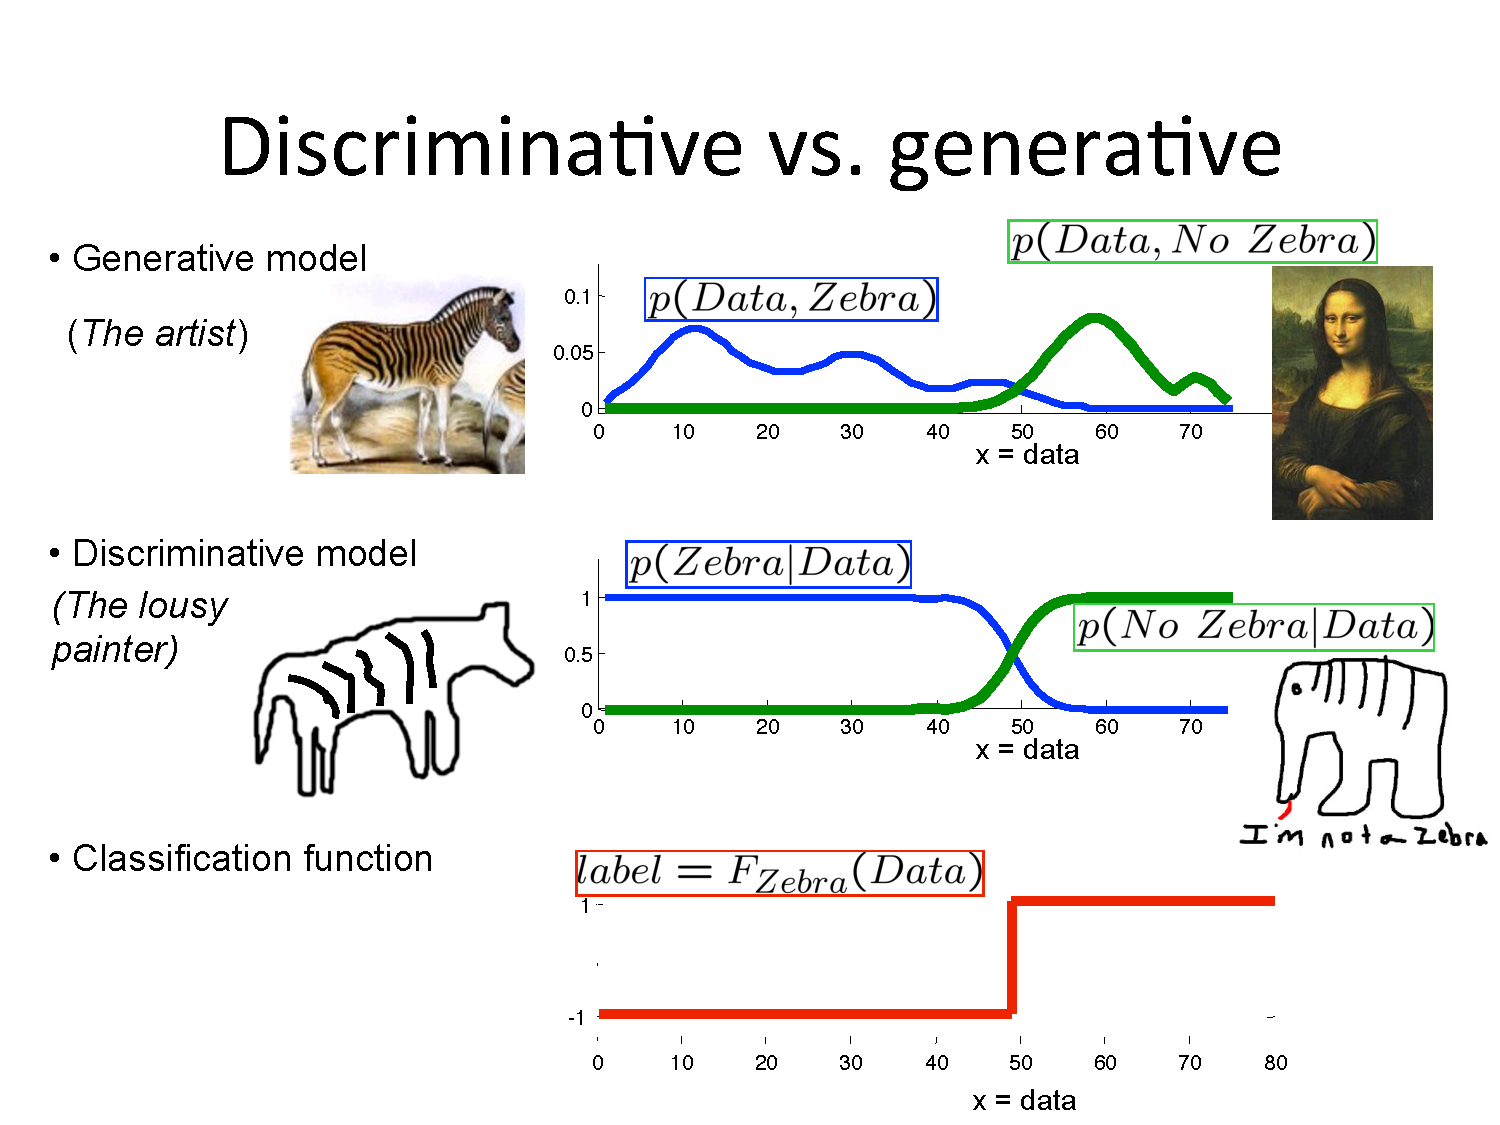
\includegraphics[width=2.5in]{figures/zebra_painting.pdf}
Why does the generative p graph max out at 0.1 and the discriminative at 1?   
    Discriminating against zebra or not zebra.  Has to sum to 1.  
    The discriminative doesn't have to sum to 1.  Many other things have to sum with it to sum to 1. 
    
 
 \subsection{Linear Classifiers}
 Inputs are feature values.  \hfill \\
 Each feature has a weight.  \hfill \\
 Sum is the activation.  activation$_w(x) = \sum_i w_i x_i = w \cdot x$  \hfill \\
 If the activation is positive, chose output class 1.  \hfill \\
 If the activation is netative, chose output class 2.  \hfill \\
 
 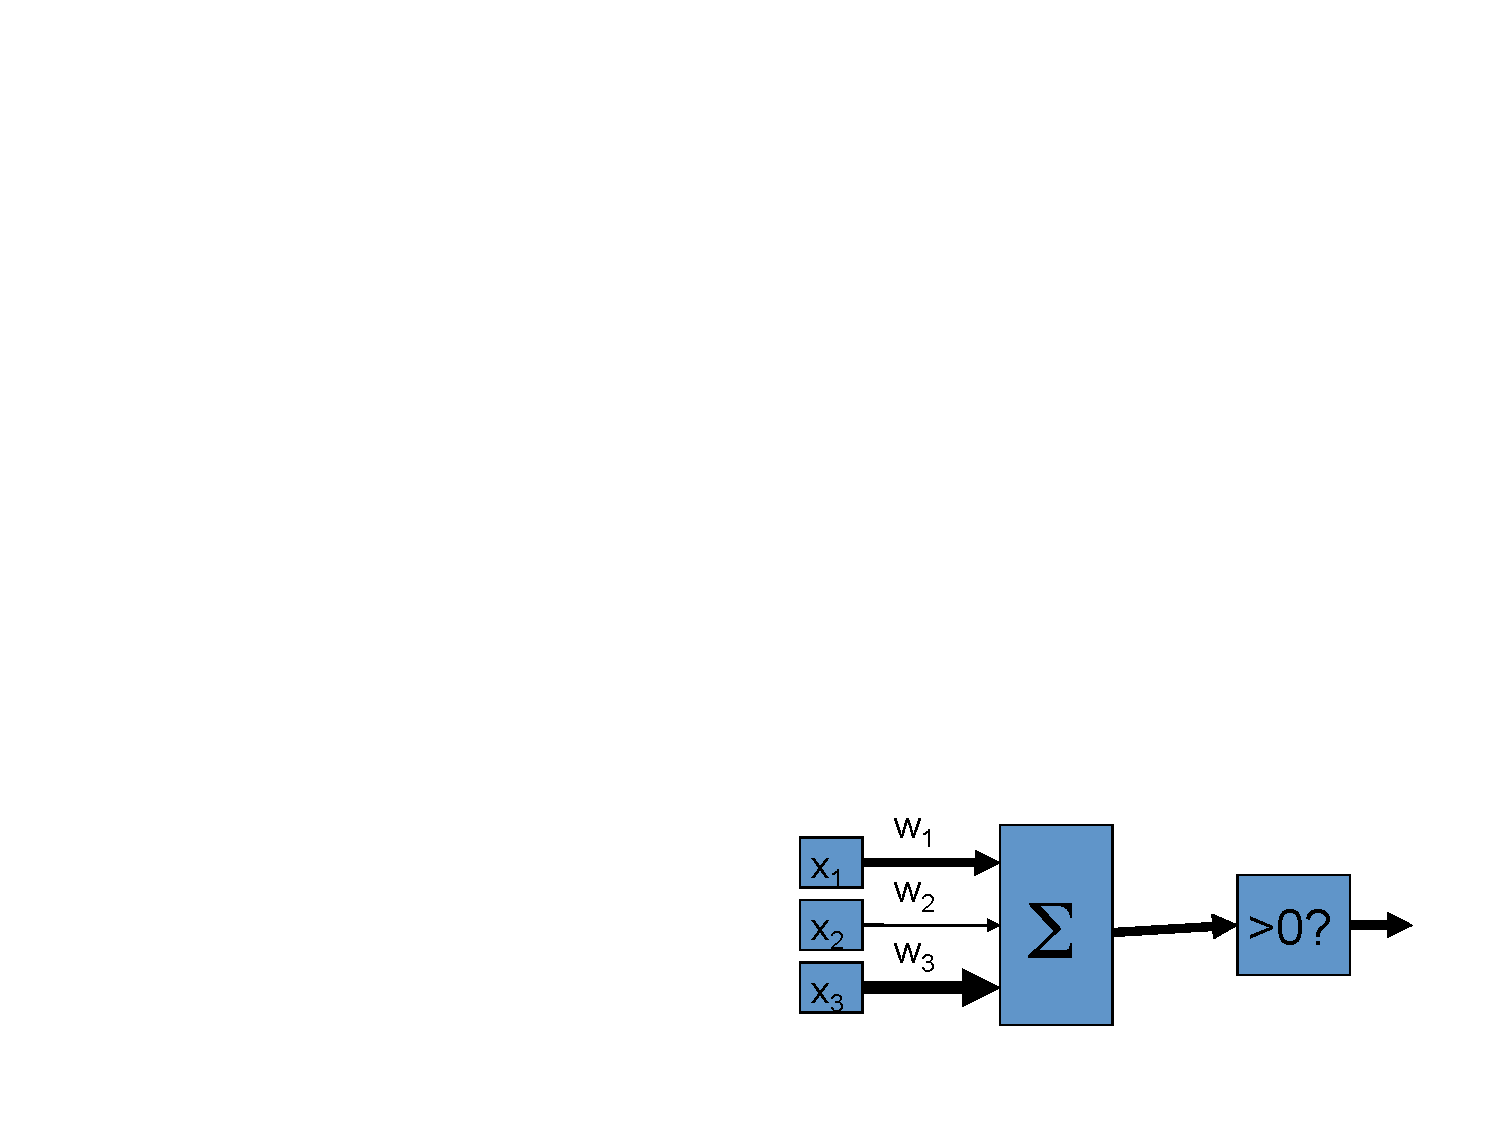
\includegraphics[width=1.5in]{figures/linear_classifier_cartoon.pdf}  \hfill \\
 
 For a binary decision rule:   \hfill \\
 In the space of feature vectors: 
 \begin{itemize}
 	\item examples are points
	\item any weight vector is a hyperplane
	\item one side corresponds to y = +1
	\item the other side corresponds to y = -1
	\item ??? The $w \cdot x = 0$ is the solution to the line.
 \end{itemize}
 
 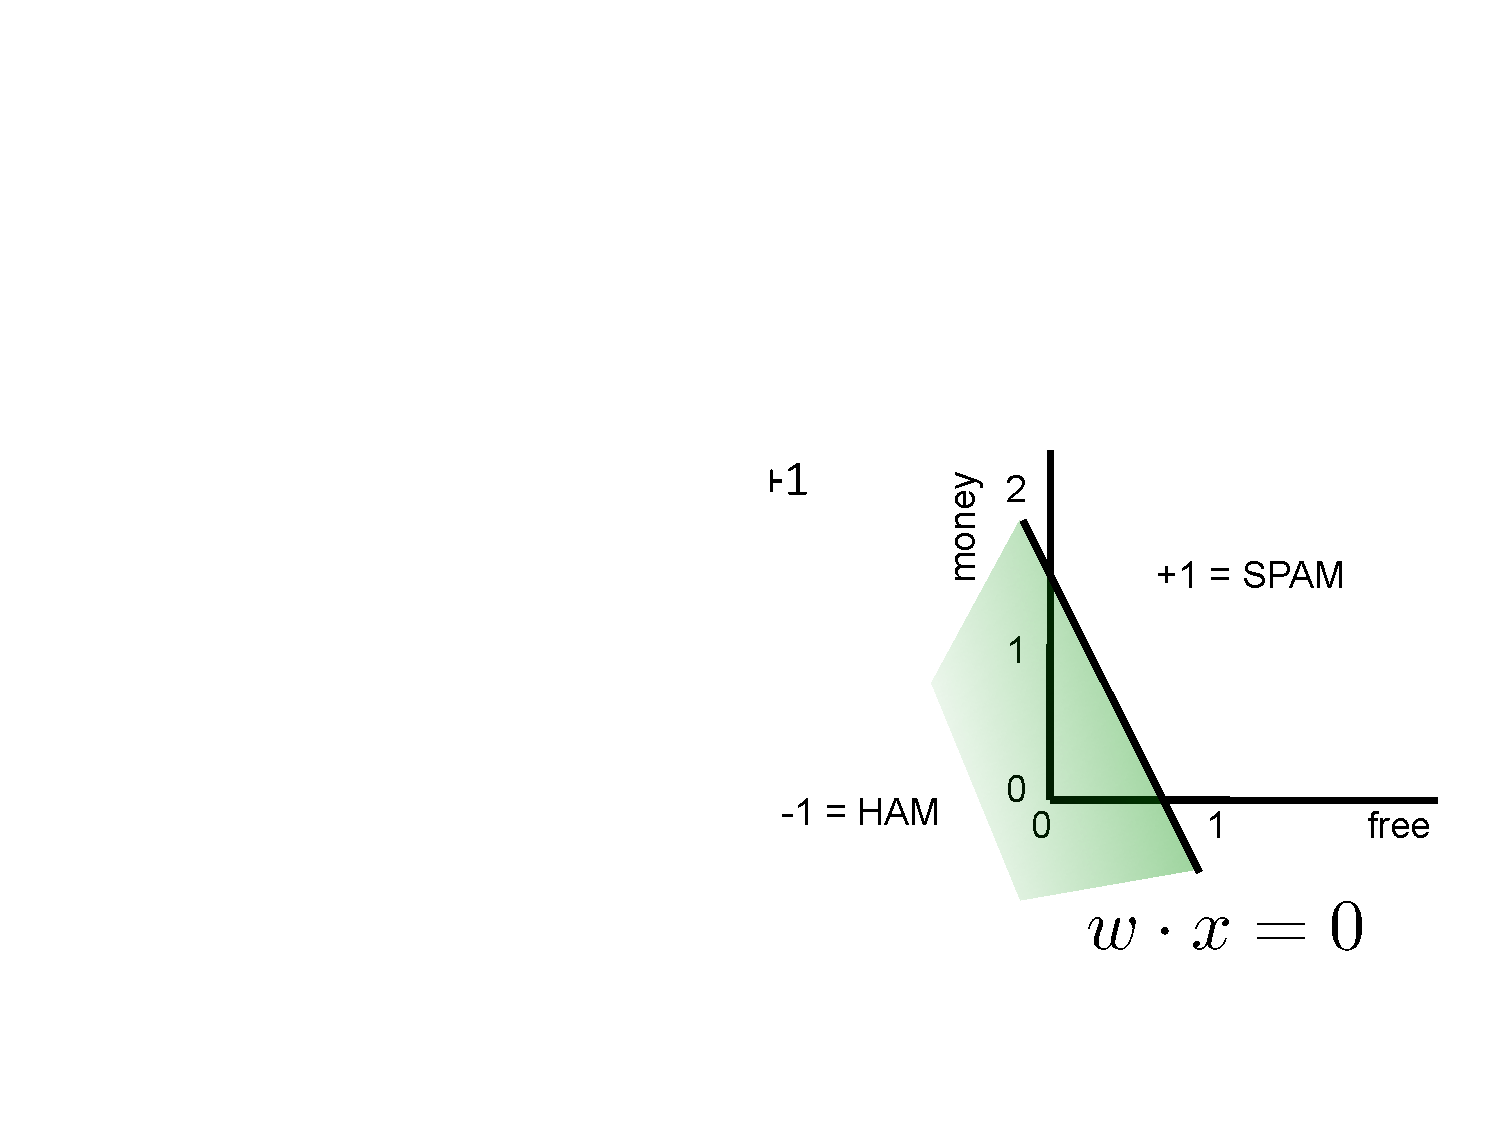
\includegraphics[width=1.5in]{figures/binary_decision_rule.pdf}
 
 \subsection{NB, LR, Perceptron}
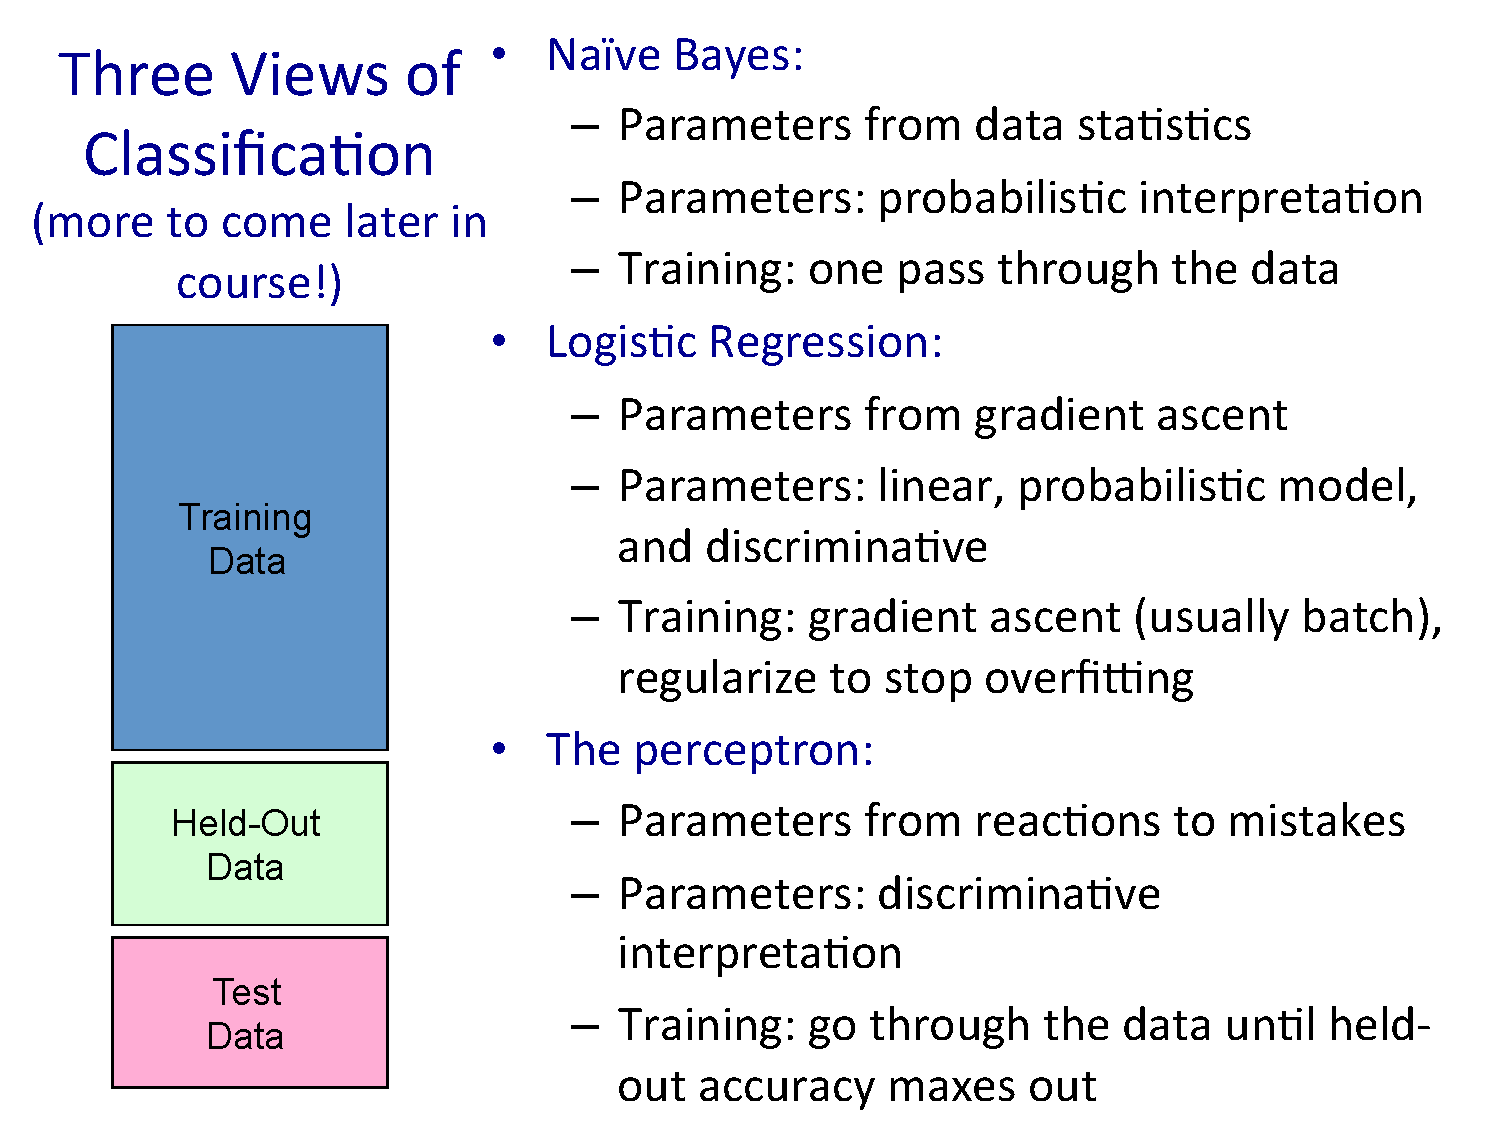
\includegraphics[width=2.5in]{figures/three_views_of_classification.pdf}

\subsection{Gradient Ascent/Descent vs Coordinate Ascent/Descent}
 We discussed gradient descent with logistic regression. \hfill \\
 We mentioned coordinate descent when getting ready to talk about EM.   \hfill \\

\subsubsection{Gradient descent}
For finding the local minimum. 
\begin{itemize}
	\item Takes steps proportional to the negative of the gradient 
		(or of the approximate gradient) of the function at the current point. 
	\item If instead one takes steps proportional to the positive of the gradient, 
		one approaches a local maximum of that function; 
		the procedure is then known as gradient ascent.
\end{itemize}	

\subsubsection{Coordinate descent}
\begin{itemize}
	\item A non-derivative optimization algorithm
	\item To find a local minimum of a function, one does line search along 
		one coordinate direction at the current point in each iteration. 
		One uses different coordinate directions cyclically throughout the procedure.
	\item Has problems with non-smooth functions 
		% https://en.wikipedia.org/wiki/Coordinate_descent
	\item Coordinate descent \textbf{does} have step size parameter. % week 10 audio
		To prevent over-shooting, you many need to take smaller steps. 
	\item  Does converge under two big assumptions: \hfill \\
		(1) fixing one works.   \hfill \\
		(2) need loss to get smaller than it was before. \hfill \\
	\item Won't always converge to global optima.
	\item For coordinate descent, you have to be extremely careful that each step reduces the loss function.
		If you can't prove that you should not use coordinate descent. 
\end{itemize}	

K-means does this: alternate between holding the assignments and the centers fixed. 




\vspace{4in}
\bigskip


\end{multicols*}
\end{document}
